\documentclass[12pt,a4paper]{article}

\usepackage[utf8]{inputenc}
\usepackage[T1]{fontenc}
\usepackage{geometry}
\geometry{margin=2.5cm}

\usepackage{graphicx}
\usepackage{float}
\usepackage{booktabs}
\usepackage{longtable}
\usepackage{array}
\usepackage{xcolor}
\usepackage{listings}
\usepackage{hyperref}
\usepackage{amsmath}
\usepackage{amssymb}
\usepackage{enumitem}
\usepackage{fancyhdr}
\usepackage{titlesec}
\usepackage{caption}
\usepackage{subcaption}
\usepackage{parskip}
\usepackage{mdframed}
\usepackage{tikz}
\usetikzlibrary{shapes.geometric, arrows.meta, positioning, fit, backgrounds}

\hypersetup{
    colorlinks=true,
    linkcolor=blue!60!black,
    urlcolor=blue!60!black,
    citecolor=blue!60!black
}

% ── Code listing style ──────────────────────────────────────────────────────
\definecolor{codebg}{RGB}{248,248,248}
\definecolor{codeframe}{RGB}{220,220,220}
\definecolor{kwcolor}{RGB}{0,0,180}
\definecolor{strcolor}{RGB}{163,21,21}
\definecolor{cmtcolor}{RGB}{0,128,0}

\lstset{
    backgroundcolor=\color{codebg},
    frame=single,
    rulecolor=\color{codeframe},
    basicstyle=\ttfamily\small,
    keywordstyle=\color{kwcolor}\bfseries,
    stringstyle=\color{strcolor},
    commentstyle=\color{cmtcolor}\itshape,
    breaklines=true,
    showstringspaces=false,
    tabsize=2,
    captionpos=b,
    numbers=left,
    numberstyle=\tiny\color{gray},
    numbersep=5pt,
    xleftmargin=15pt
}

\lstdefinelanguage{Solidity}{
    keywords={pragma, solidity, contract, function, returns, uint256, uint8,
              address, bool, bytes32, bytes, mapping, struct, enum, event,
              modifier, require, revert, emit, view, pure, payable, external,
              public, private, internal, override, virtual, memory, storage,
              calldata, if, else, for, while, return, true, false, new,
              delete, this, msg, block, tx, address, type},
    comment=[l]{//},
    morecomment=[s]{/*}{*/},
    morestring=[b]",
    sensitive=true
}

\lstdefinelanguage{JavaScript}{
    keywords={const, let, var, function, async, await, return, if, else,
              for, while, class, new, this, true, false, null, undefined,
              require, module, exports, import, from, of, in, throw, try,
              catch, finally},
    comment=[l]{//},
    morecomment=[s]{/*}{*/},
    morestring=[b]",
    morestring=[b]`,
    sensitive=true
}

% ── Page style ───────────────────────────────────────────────────────────────
\pagestyle{fancy}
\fancyhf{}
\fancyhead[L]{\small Decentralized Logistics Marketplace}
\fancyhead[R]{\small CS438 Final Report}
\fancyfoot[C]{\thepage}

% ── Section formatting ────────────────────────────────────────────────────────
\titleformat{\section}{\Large\bfseries}{{\thesection.}}{0.5em}{}[\titlerule]
\titleformat{\subsection}{\large\bfseries}{{\thesubsection}}{0.5em}{}

% ── Invariant box ─────────────────────────────────────────────────────────────
\newmdenv[
    backgroundcolor=blue!5,
    linecolor=blue!40,
    linewidth=1.2pt,
    innerleftmargin=10pt,
    innerrightmargin=10pt,
    innertopmargin=6pt,
    innerbottommargin=6pt
]{invariantbox}

\newmdenv[
    backgroundcolor=red!5,
    linecolor=red!40,
    linewidth=1.2pt,
    innerleftmargin=10pt,
    innerrightmargin=10pt,
    innertopmargin=6pt,
    innerbottommargin=6pt
]{attackbox}

% ─────────────────────────────────────────────────────────────────────────────
\begin{document}

% ── Title page ────────────────────────────────────────────────────────────────
\begin{titlepage}
\centering
\vspace*{2cm}
{\Huge\bfseries Decentralized Logistics Marketplace\par}
\vspace{0.4cm}
{\Large Final Report — CS438 / SEC532, Spring 2026\par}
\vspace{2cm}
{\large
Ekin Gülhan \hspace{0.3cm} (34028) \\[0.3em]
Aziz Derin Ebil \hspace{0.3cm} (34332) \\[0.3em]
Mert Hasan Aslan \hspace{0.3cm} (32421)
\par}
\vspace{1.5cm}
{\large \today\par}
\vspace{3cm}

\begin{abstract}
We present a permissionless, trust-minimised logistics marketplace running on the Ethereum Virtual Machine. Sellers post delivery requests on-chain; couriers compete by placing bids backed by a shared staking pool; an autonomous seller-side agent selects the best bid under on-chain policy limits; a per-delivery escrow vault holds the buyer's payment and releases it only after a sensor-gated mailbox agent confirms physical delivery. The system enforces all critical payment invariants in Solidity — no off-chain party can override them. We document the architecture, on-chain invariants, agent design, security model, test suite, and testnet deployment.
\end{abstract}
\end{titlepage}

\tableofcontents
\newpage

% =============================================================================
\section{Introduction}
% =============================================================================

Existing courier services are centralised: customers trust a single company to carry their package, handle disputes, and pay couriers. Our goal is to remove that central intermediary while retaining the same end-to-end guarantees — payment released only after delivery, couriers penalised for failure, and no party able to cheat without economic consequences.

The project belongs to the \emph{Agentic Payments} theme. An agent (the seller's autonomous program) observes on-chain bid data, applies a scoring policy, and executes blockchain transactions on the seller's behalf. A second agent (the buyer's smart mailbox) autonomously confirms physical delivery. Both agents operate under explicit, on-chain payment policies: the smart contracts will revert any action that violates the rules, regardless of what the agents decide off-chain.

\subsection{What Is Original}

\begin{enumerate}
    \item \textbf{Per-delivery escrow vault spawned by the registry.} Each accepted bid atomically deploys a fresh \texttt{DeliveryVault} instance. No two deliveries share state; a catastrophic failure in one vault cannot bleed into another.
    \item \textbf{Pooled staking with capacity invariants.} Couriers lock funds into a shared pool, enabling them to cover high-value deliveries without per-delivery deposits. The invariant $\texttt{activeValue} \leq \texttt{totalStake}$ is enforced on every reserve and withdrawal.
    \item \textbf{Sensor-gated mailbox agent.} The buyer's mailbox holds a dedicated signing key inside a simulated secure element. It will not call \texttt{confirmDelivery} unless onboard sensors pass and a rate-limit is satisfied.
    \item \textbf{On-chain agent policy enforcement.} The seller registers \texttt{(maxPrice, deadlineBuffer, coSignThreshold)} in the registry. \texttt{acceptBidByAgent} reverts if any limit is violated — a hallucinating LLM cannot accept an out-of-policy bid.
    \item \textbf{Preimage binding of pickup/dropoff codes.} Codes commit to $\mathtt{keccak256}(\mathit{code} \| \mathit{deliveryId} \| \mathit{nonce})$, not just the code. A code revealed for delivery A is cryptographically useless for delivery B.
\end{enumerate}

% =============================================================================
\section{System Architecture}
% =============================================================================

\subsection{Components Overview}

The system has three layers:

\begin{itemize}
    \item \textbf{On-chain (EVM):} \texttt{MarketplaceRegistry}, \texttt{DeliveryVault}, \texttt{StakingPool}
    \item \textbf{Off-chain agents:} Seller Agent, Mailbox Agent
    \item \textbf{Client interfaces:} Seller CLI/GUI, Courier CLI, Buyer CLI/GUI
\end{itemize}

\begin{figure}[H]
\centering
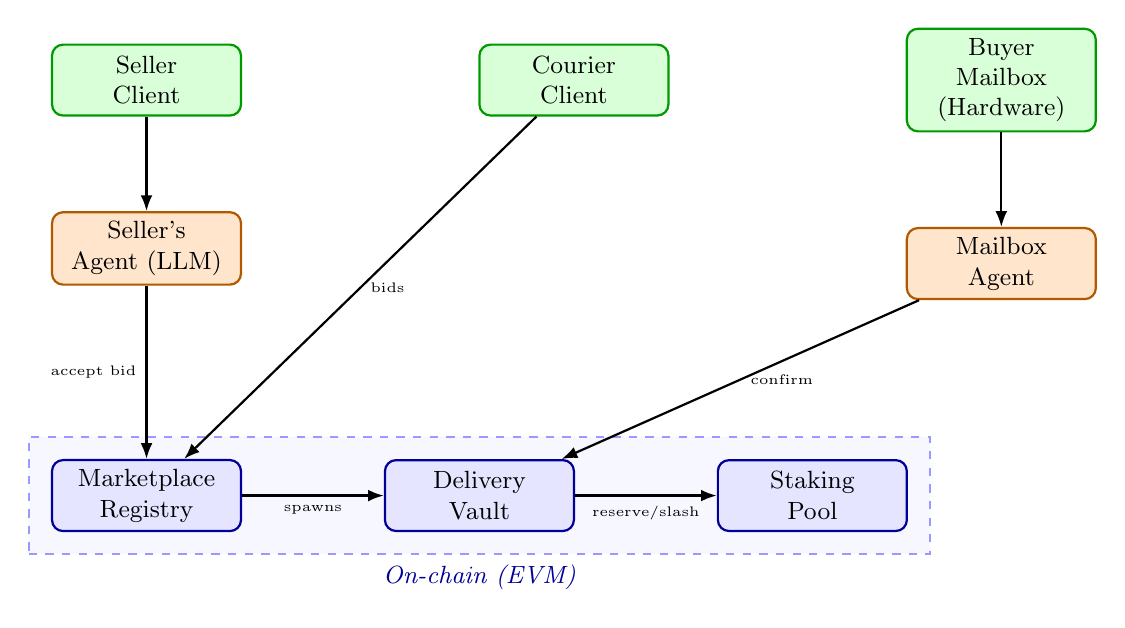
\begin{tikzpicture}[
    node distance=1.4cm and 2.0cm,
    box/.style={rectangle, rounded corners=4pt, draw, thick, minimum width=2.4cm, minimum height=0.9cm, align=center, font=\small},
    greenbox/.style={box, fill=green!15, draw=green!60!black},
    orangebox/.style={box, fill=orange!20, draw=orange!70!black},
    bluebox/.style={box, fill=blue!10, draw=blue!60!black},
    arr/.style={-{Latex[length=2mm]}, thick}
]
% Clients
\node[greenbox] (seller)   {Seller\\Client};
\node[greenbox, right=3cm of seller] (courier) {Courier\\Client};
\node[greenbox, right=3cm of courier] (buyer)  {Buyer\\Mailbox\\(Hardware)};

% Agents
\node[orangebox, below=1.2cm of seller]  (sagent) {Seller's\\Agent (LLM)};
\node[orangebox, below=1.2cm of buyer]   (magent) {Mailbox\\Agent};

% Contracts
\node[bluebox, below=2.2cm of sagent]    (registry) {Marketplace\\Registry};
\node[bluebox, right=1.8cm of registry]  (vault)    {Delivery\\Vault};
\node[bluebox, right=1.8cm of vault]     (pool)     {Staking\\Pool};

% Arrows
\draw[arr] (seller)  -- (sagent);
\draw[arr] (buyer)   -- (magent);
\draw[arr] (courier) -- (registry) node[midway, right, font=\tiny] {bids};
\draw[arr] (sagent)  -- (registry) node[midway, left,  font=\tiny] {accept bid};
\draw[arr] (magent)  -- (vault)    node[midway, right, font=\tiny] {confirm};
\draw[arr] (registry)-- (vault)    node[midway, below, font=\tiny] {spawns};
\draw[arr] (vault)   -- (pool)     node[midway, below, font=\tiny] {reserve/slash};

% On-chain box
\begin{pgfonlayer}{background}
  \node[draw=blue!40, dashed, thick, fill=blue!3,
        fit=(registry)(vault)(pool),
        inner sep=8pt, label={[blue!60!black, font=\small\itshape]below:On-chain (EVM)}]
       (onchain) {};
\end{pgfonlayer}
\end{tikzpicture}
\caption{System architecture. Green nodes are human-controlled clients; orange nodes are autonomous agents; blue nodes are Solidity contracts.}
\label{fig:arch}
\end{figure}

\subsection{Delivery Lifecycle}

\begin{enumerate}
    \item Seller posts a delivery request on \texttt{MarketplaceRegistry} with declared value, max price, deadline, buyer/mailbox addresses, and pool reference.
    \item Seller publishes pickup and dropoff code hashes (locked permanently after this step).
    \item Couriers place bids (price, promised delivery time, reputation score).
    \item Seller's agent waits for the bid window, ranks bids, and calls \texttt{acceptBidByAgent}. The registry atomically deploys a \texttt{DeliveryVault} and reserves the courier's stake in the pool.
    \item Buyer funds the vault.
    \item Courier picks up the package and calls \texttt{pickup(code, nonce)} on the vault.
    \item Courier delivers and reveals the dropoff code to the mailbox.
    \item Mailbox agent verifies sensors, calls \texttt{confirmDelivery(code, nonce)}.
    \item After the dispute window, \texttt{finalizeDelivered} releases payment to the courier and releases pool stake.
\end{enumerate}

\begin{figure}[H]
\centering
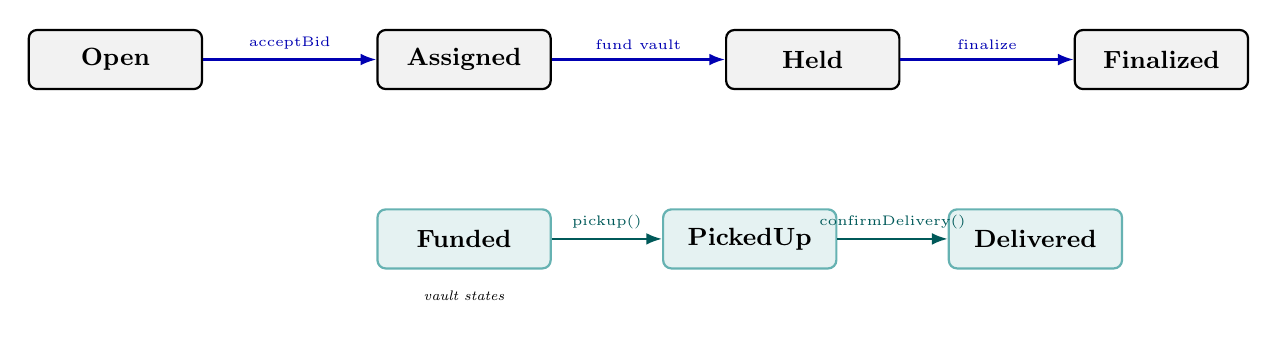
\begin{tikzpicture}[
    state/.style={rectangle, rounded corners=3pt, draw, thick, minimum width=2.2cm, minimum height=0.75cm, align=center, font=\small\bfseries, fill=gray!10},
    arr/.style={-{Latex[length=2mm]}, thick, blue!70!black},
    lab/.style={font=\tiny, midway, above}
]
\node[state] (open)     {Open};
\node[state, right=2.2cm of open]     (assigned) {Assigned};
\node[state, right=2.2cm of assigned] (held)     {Held};
\node[state, right=2.2cm of held]     (final)    {Finalized};

\draw[arr] (open)     -- (assigned) node[lab]{acceptBid};
\draw[arr] (assigned) -- (held)     node[lab]{fund vault};
\draw[arr] (held)     -- (final)    node[lab]{finalize};

% Vault states below
\node[state, fill=teal!10, draw=teal!60, below=1.5cm of assigned] (funded)    {Funded};
\node[state, fill=teal!10, draw=teal!60, right=1.4cm of funded]   (pickedup)  {PickedUp};
\node[state, fill=teal!10, draw=teal!60, right=1.4cm of pickedup] (delivered) {Delivered};

\draw[arr, teal!70!black] (funded)    -- (pickedup)  node[lab]{pickup()};
\draw[arr, teal!70!black] (pickedup)  -- (delivered) node[lab]{confirmDelivery()};

\node[font=\tiny\itshape, below=0.15cm of funded] {vault states};
\end{tikzpicture}
\caption{Registry stage machine (top) and vault state machine (bottom). Neither can be rewound or skipped.}
\label{fig:states}
\end{figure}

% =============================================================================
\section{Smart Contracts}
% =============================================================================

\subsection{MarketplaceRegistry}

\texttt{MarketplaceRegistry} is the entry point for the entire system. It stores delivery requests and bids, enforces access control, and acts as a factory for \texttt{DeliveryVault} instances.

\textbf{Key data structures:}

\begin{lstlisting}[language=Solidity, caption=Request and Bid structs in MarketplaceRegistry.sol]
struct Request {
    address seller;
    uint256 declaredValue;    // package value for staking cap
    uint256 maxPrice;         // seller's budget for courier fee
    uint256 maxDeadline;      // unix delivery deadline
    uint256 bidDeadline;      // unix time bids close
    address buyer;
    address mailbox;
    StakingPool pool;
    bytes32 pickupHash;
    bytes32 dropoffHash;
    bool    preferTrusted;    // passed to agent for scoring
    uint256 disputeWindow;    // forwarded to vault
    Stage   stage;            // Open -> Assigned -> Held -> Finalized
    uint256 acceptedBidIndex;
    address vault;
    uint256 createdAt;
}

struct Bid {
    address courier;
    address payout;           // locked at acceptance
    uint256 price;
    uint256 promisedTime;     // unix timestamp
    uint256 reputationE4;     // [0, 10000] = [0%, 100%]
    uint64  submittedAt;
    bool    withdrawn;
}
\end{lstlisting}

\textbf{Critical enforcement points:}

\begin{itemize}
    \item \texttt{openRequest}: generates a unique delivery ID from \texttt{keccak256(seller, salt, block.timestamp)}.
    \item \texttt{placeBid}: verifies courier is a pool member and that \texttt{pool.freeCapacityFor(courier) $\geq$ declaredValue}.
    \item \texttt{publishHashes}: callable only once; hashes are locked permanently after this call.
    \item \texttt{acceptBid}: moves stage Open $\to$ Assigned; deploys a \texttt{DeliveryVault}; calls \texttt{pool.reserve()}.
    \item \texttt{acceptBidByAgent}: same as \texttt{acceptBid} but additionally checks agent policy (see Section~\ref{sec:policy}).
\end{itemize}

\subsection{DeliveryVault}

Each accepted delivery gets its own \texttt{DeliveryVault}. The vault holds the buyer's payment and enforces all payment conditions.

\begin{lstlisting}[language=Solidity, caption=Core enforcement in DeliveryVault.sol (simplified)]
function pickup(bytes calldata code, bytes32 nonce)
    external nonReentrant notFinalized
{
    require(msg.sender == courier, "not courier");
    require(isFunded, "not funded");
    bytes32 h = keccak256(abi.encodePacked(code, deliveryId, nonce));
    require(h == pickupHash, "bad pickup preimage");
    require(block.timestamp <= pickupDeadline, "pickup timeout");
    s = VaultState.PickedUp;
    pool.release(courier, declaredValue); // free reserved capacity
    emit PickedUp(courier, block.timestamp);
}

function confirmDelivery(bytes calldata code, bytes32 nonce)
    external nonReentrant notFinalized
{
    require(msg.sender == mailbox, "not mailbox");
    bytes32 h = keccak256(abi.encodePacked(code, deliveryId, nonce));
    require(h == dropoffHash, "bad dropoff preimage");
    s = VaultState.Delivered;
    deliveredAt = block.timestamp;
    emit Delivered(mailbox, block.timestamp);
}

function finalizeDelivered() external nonReentrant notFinalized {
    require(s == VaultState.Delivered, "not delivered");
    require(block.timestamp >= deliveredAt + disputeWindow, "dispute window");
    finalized = true;             // set BEFORE external call (CEI)
    uint256 fee = courierFee;
    (bool ok,) = payout.call{value: fee}("");
    require(ok, "payout failed");
    emit Finalized(payout, fee);
}
\end{lstlisting}

\textbf{Timeout paths:}
\begin{itemize}
    \item \texttt{refundOnPickupTimeout}: if courier has not called \texttt{pickup} before \texttt{pickupDeadline}, buyer gets their payment back; pool stake is released (courier was present but failed).
    \item \texttt{slashOnDropoffTimeout}: if courier called \texttt{pickup} but failed to deliver before \texttt{dropoffDeadline}, pool slashes the courier's stake and pays it to the buyer.
\end{itemize}

\subsection{StakingPool}

\texttt{StakingPool} is a shared collateral fund. Multiple couriers contribute, and the pool backs each courier's active deliveries up to the pool's capacity.

\textbf{Core invariant:}

\begin{invariantbox}
\[
\texttt{activeValue} \leq \texttt{totalStake}
\]
This is checked on every \texttt{reserve()} call (when a bid is accepted) and on every \texttt{requestWithdraw()} call. No delivery can be assigned that would push total active value above total stake.
\end{invariantbox}

\textbf{Per-member cap:}
Each member's total reserved value cannot exceed \texttt{memberCapBps / 10000 $\times$ contribution}. This limits a single colluding courier's leverage over the pool.

\textbf{Withdrawal delay:}
\begin{lstlisting}[language=Solidity, caption=Withdrawal delay in StakingPool.sol (simplified)]
function requestWithdraw(uint256 amount) external {
    MemberInfo storage m = members[msg.sender];
    require(m.isMember, "not member");
    require(m.contribution - m.reserved >= amount, "would breach cap");
    // activeValue <= totalStake must hold after withdrawal
    require(activeValue <= totalStake - amount, "would break invariant");
    m.withdrawReqAt  = block.timestamp;
    m.withdrawReqAmt = amount;
}

function finalizeWithdraw() external {
    MemberInfo storage m = members[msg.sender];
    require(m.withdrawReqAmt > 0, "no pending");
    require(block.timestamp >= m.withdrawReqAt + withdrawalDelay, "too soon");
    uint256 amt = m.withdrawReqAmt;
    m.withdrawReqAmt = 0;
    totalStake -= amt;
    m.contribution -= amt;
    (bool ok,) = msg.sender.call{value: amt}("");
    require(ok, "transfer failed");
}
\end{lstlisting}

The withdrawal delay prevents a pool member from racing to exit the moment they sense a fellow courier is about to fail a high-value delivery.

% =============================================================================
\section{On-chain Payment Policy and Agent Safety}
\label{sec:policy}
% =============================================================================

\subsection{Agent Policy Registration}

The seller calls \texttt{setAgentPolicy} once to register a session key and its limits:

\begin{lstlisting}[language=Solidity, caption=Agent policy storage]
struct AgentPolicy {
    address agentAddr;
    uint256 maxPrice;          // agent cannot accept above this
    uint256 deadlineBuffer;    // bid.promisedTime must be >= now + buffer
    uint256 coSignThreshold;   // auto-accept only if declaredValue <= this
    bool    isSet;
}
mapping(address => AgentPolicy) public agentPolicies; // seller => policy
\end{lstlisting}

\subsection{acceptBidByAgent Enforcement}

\begin{lstlisting}[language=Solidity, caption=Policy enforcement in acceptBidByAgent]
function acceptBidByAgent(bytes32 deliveryId, uint256 bidIndex)
    external returns (address vault)
{
    Request storage req = requests[deliveryId];
    AgentPolicy storage pol = agentPolicies[req.seller];
    require(pol.isSet, "no agent policy");
    require(msg.sender == pol.agentAddr, "not agent");

    Bid storage bid = bids[deliveryId][bidIndex];
    require(bid.price <= pol.maxPrice, "price > maxPrice");
    require(bid.promisedTime >= block.timestamp + pol.deadlineBuffer,
            "insufficient deadline buffer");
    require(req.declaredValue <= pol.coSignThreshold,
            "co-sign required: value above threshold");

    return _acceptBid(deliveryId, bidIndex);
}
\end{lstlisting}

If \texttt{declaredValue > coSignThreshold}, \texttt{acceptBidByAgent} reverts on-chain. The off-chain agent detects this beforehand and emits a \texttt{co-sign-needed} A2A message — the human seller must call \texttt{acceptBid} with their master key.

\subsection{Scoring Formula}

The seller agent ranks bids using:

\[
\text{score}_i = \frac{r_i^{\,\alpha}}{t_i \cdot p_i}
\]

\begin{center}
\begin{tabular}{cll}
\toprule
Symbol & Meaning & Range \\
\midrule
$r_i$ & Courier reputation factor & $[0,1]$ (stored as basis points / 10000) \\
$t_i$ & Seconds until courier's promised delivery & $> 0$ \\
$p_i$ & Price asked (wei) & $> 0$ \\
$\alpha$ & Reputation weight & $0$ if \textit{preferTrusted} unchecked; $1.5$ otherwise \\
\bottomrule
\end{tabular}
\end{center}

Hard filters (maxPrice, maxDeadline) eliminate ineligible bids \emph{before} scoring. The LLM commentary (via OpenAI GPT-4o-mini) can explain the winner but cannot change it — the decision is fully determined by the formula before the model is consulted.

% =============================================================================
\section{Agent Implementation}
% =============================================================================

\subsection{Seller Agent}

\texttt{agents/seller\_agent.js} is a Node.js process that:

\begin{enumerate}
    \item \textbf{Ingests:} on-chain bids for a given \texttt{deliveryId}, fetched after the bid window closes.
    \item \textbf{Decides:} runs \texttt{SellerAgent.rank()} from \texttt{seller\_agent\_core.js} — deterministic, no LLM involved in the decision.
    \item \textbf{Executes:} calls \texttt{registry.acceptBidByAgent(deliveryId, winnerIndex)} via ethers.js.
    \item \textbf{Verifies:} parses the \texttt{BidAccepted} event log; logs the vault address.
    \item \textbf{Escalates:} if \texttt{declaredValue > coSignThreshold}, emits a \texttt{co-sign-needed} A2A message instead of sending the transaction.
\end{enumerate}

\textbf{A2A protocol.} The agent speaks a JSON-line Agent-to-Agent protocol (documented in \texttt{docs/A2A.md}) over stdin/stdout. Supported intents:

\begin{center}
\begin{tabular}{lll}
\toprule
Intent & Direction & Purpose \\
\midrule
\texttt{bid-discuss}    & courier $\to$ seller & Ask if a proposed bid would rank well before paying gas \\
\texttt{bid-confirm}    & courier $\to$ seller & Notify agent that an on-chain bid was placed \\
\texttt{co-sign-needed} & seller $\to$ human   & Escalate: value above coSignThreshold \\
\texttt{rank-explain}   & any $\to$ seller     & Debug: fetch full ranking of open bids \\
\bottomrule
\end{tabular}
\end{center}

\subsection{Mailbox Agent}

\texttt{agents/mailbox\_agent.js} simulates the buyer's physical smart mailbox:

\begin{enumerate}
    \item \textbf{Ingests:} dropoff code + nonce presented by the courier at the physical mailbox.
    \item \textbf{Decides:} reads sensor data (simulated package weight, lid state) and checks rate limit (60 s between confirmations).
    \item \textbf{Executes:} calls \texttt{vault.confirmDelivery(code, nonce)} with the mailbox key.
    \item \textbf{Verifies:} waits for transaction confirmation; logs receipt hash.
\end{enumerate}

The mailbox key has exactly one on-chain capability: calling \texttt{confirmDelivery}. It cannot transfer funds, cancel requests, or touch any other contract state.

\begin{lstlisting}[language=JavaScript, caption=Sensor check in mailbox\_agent.js]
function readSensors() {
  const weightGrams = Number(process.env.MAILBOX_WEIGHT_OVERRIDE ?? 250);
  const lidClosed   = process.env.MAILBOX_LID_OVERRIDE !== "open";
  // Weight > 50g AND lid closed = package is present
  return { ok: weightGrams > 50 && lidClosed, weightGrams, lidClosed };
}
\end{lstlisting}

% =============================================================================
\section{Security Model}
% =============================================================================

\subsection{Trust Boundaries}

\begin{center}
\begin{tabular}{p{4.5cm}p{9.5cm}}
\toprule
Boundary & Risk \\
\midrule
Agent $\leftrightarrow$ Smart Contract &
LLM may hallucinate bid rankings or miscompute policy. Mitigated by on-chain policy enforcement — any out-of-policy transaction reverts. \\
\addlinespace
Physical Mailbox $\leftrightarrow$ Blockchain &
Hardest boundary. Blockchain cannot verify physical reality; it only verifies a key signature. Mailbox can be tampered; sensors can be fooled with a decoy package. \\
\addlinespace
Couriers $\leftrightarrow$ Staking Pool &
Malicious courier imposes slashing externalities on honest pool members. Withdrawal delay and per-member cap limit damage. \\
\addlinespace
Seller $\leftrightarrow$ Buyer (off-chain) &
Pickup/dropoff codes are exchanged off-chain. If this channel is eavesdropped, an attacker obtains the codes. On-chain mitigation: codes are bound to \texttt{deliveryId}; a leaked code is useless on any other delivery. \\
\bottomrule
\end{tabular}
\end{center}

\subsection{Attack Scenarios}

\begin{attackbox}
\textbf{Attack 1: Malicious or buggy LLM accepts wrong bid.}

\textit{Scenario:} The LLM miscomputes the $r/(t \cdot p)$ ranking and calls \texttt{acceptBidByAgent} on a courier the seller would not have chosen.

\textit{Mitigation:} Two-layer defence. First, \texttt{acceptBidByAgent} checks \texttt{price $\leq$ maxPrice} and \texttt{promisedTime $\geq$ now + deadlineBuffer} on-chain; any violation reverts. Second, if \texttt{declaredValue > coSignThreshold} the agent call reverts unconditionally — the human seller must co-sign with their master key. \textit{Tested:} \texttt{rejects agent bid above maxPrice}, \texttt{rejects agent acceptance above coSignThreshold}.
\end{attackbox}

\begin{attackbox}
\textbf{Attack 2: Pool member exits right before a slash.}

\textit{Scenario:} A pool member senses that a fellow courier is about to fail a high-value delivery. They call \texttt{requestWithdraw} and immediately \texttt{finalizeWithdraw} before the slash arrives, leaving remaining members to absorb their share.

\textit{Mitigation:} \texttt{finalizeWithdraw} reverts unless \texttt{block.timestamp $\geq$ withdrawReqAt + withdrawalDelay}. The delay must be longer than the maximum dropoff timeout of any active delivery the member backs. Slashes during the delay window still draw from the requester's balance. \textit{Tested:} \texttt{enforces withdrawal delay}.
\end{attackbox}

\begin{attackbox}
\textbf{Attack 3: Collusion between seller, courier, and buyer to defraud the pool.}

\textit{Scenario:} Colluding parties post a fake high-value delivery. The courier "fails" it, the pool is slashed, funds flow to the colluding buyer.

\textit{Mitigation:} Per-member reservation cap (\texttt{memberCapBps}) limits each member's leverage to a fraction of their own contribution. Pool admission requires operator approval (\texttt{admitMember}). Slash history is exposed on-chain via \texttt{getCourierStats} for external monitoring. An insurance-fee reserve is acknowledged in the design but not yet implemented.
\end{attackbox}

\begin{attackbox}
\textbf{Attack 4: Reentrancy on payout or refund.}

\textit{Scenario:} The courier's payout address is a malicious contract that re-enters \texttt{finalizeDelivered} before \texttt{finalized = true} is set.

\textit{Mitigation:} Checks-effects-interactions pattern: \texttt{finalized = true} is set before any external call. All fund-moving functions carry \texttt{nonReentrant}. Payout address is locked at bid acceptance time. \textit{Tested:} \texttt{rejects a second payout attempt}.
\end{attackbox}

\begin{attackbox}
\textbf{Attack 5: Mailbox spoofing / compromised secure element.}

\textit{Scenario:} Attacker extracts the mailbox private key and confirms a fake delivery.

\textit{Mitigation:} Preimage binding: even with the mailbox key, the attacker must supply the correct \texttt{(code, nonce)} pair such that \texttt{keccak256(code \| deliveryId \| nonce) = dropoffHash}. Without the off-chain dropoff code (known only to seller and buyer), this is computationally infeasible. Additionally, a dispute window between \texttt{Delivered} and \texttt{Finalized} lets the buyer's primary key freeze payout. \textit{Tested:} \texttt{rejects an incorrect preimage}, \texttt{allows buyer to dispute and arbiter to refund}.

\begin{figure}[H]
    \centering
    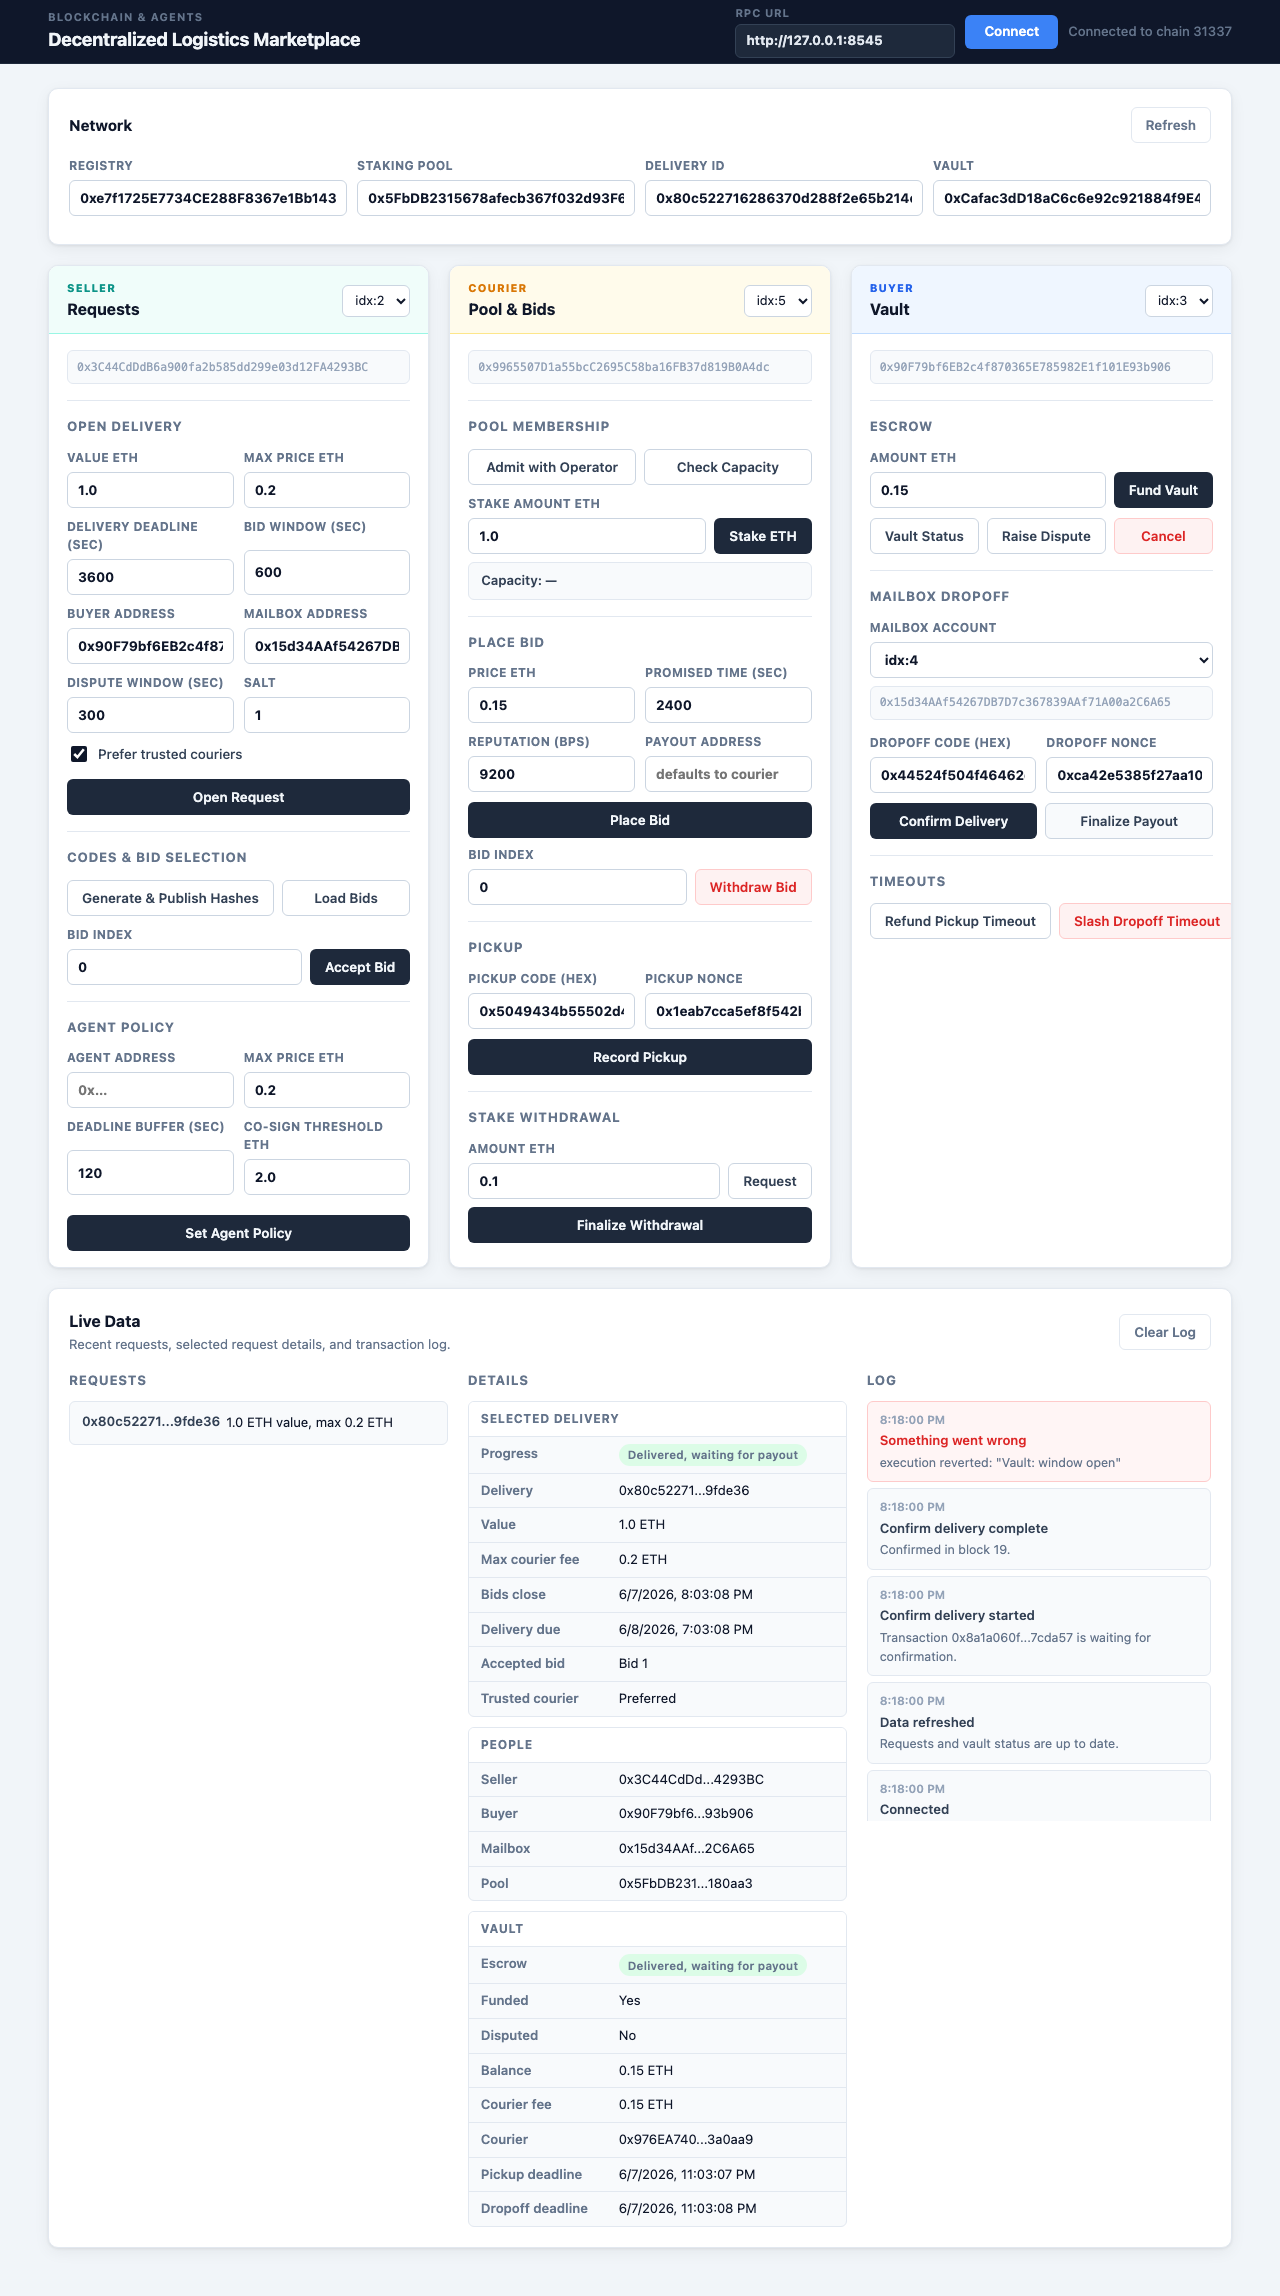
\includegraphics[width=0.75\linewidth]{screenshots/10b-dispute-window-open.png}
    \caption{Dispute window open after mailbox confirmation — the Raise Dispute button is active and the vault is in \texttt{Delivered} state pending the 60-second window.}
    \label{fig:dispute}
\end{figure}
\end{attackbox}

% =============================================================================
\section{Test Suite}
% =============================================================================

All 14 tests pass against a fresh in-process Hardhat chain. The test suite covers the full happy path and every documented attack scenario.

\begin{center}
\begin{tabular}{lll}
\toprule
Category & Test name & Result \\
\midrule
\multirow{2}{*}{Happy path}
 & seller $\to$ bid $\to$ accept $\to$ fund $\to$ pickup $\to$ confirm $\to$ payout & \checkmark \\
 & releases capacity correctly across multiple sequential deliveries & \checkmark \\
\addlinespace
\multirow{2}{*}{Timeouts}
 & refunds the buyer on pickup timeout & \checkmark \\
 & slashes the courier on dropoff timeout & \checkmark \\
\addlinespace
\multirow{3}{*}{StakingPool invariants}
 & rejects bids when courier lacks pool capacity & \checkmark \\
 & blocks withdraw that would breach member-cap on reserved value & \checkmark \\
 & enforces withdrawal delay & \checkmark \\
\addlinespace
\multirow{2}{*}{Agent session-key safety}
 & rejects agent bid above maxPrice & \checkmark \\
 & rejects agent acceptance above coSignThreshold & \checkmark \\
\addlinespace
\multirow{2}{*}{Preimage binding}
 & rejects a pickup code reused across deliveries & \checkmark \\
 & rejects an incorrect preimage & \checkmark \\
\addlinespace
\multirow{2}{*}{Dispute window}
 & allows buyer to dispute and arbiter to refund & \checkmark \\
 & finalizes after dispute window if no dispute filed & \checkmark \\
\addlinespace
Double-finalize guard
 & rejects a second payout attempt & \checkmark \\
\bottomrule
\multicolumn{2}{r}{\textbf{Total}} & \textbf{14 / 14} \\
\bottomrule
\end{tabular}
\end{center}

In addition, 12 Playwright end-to-end UI tests verify the browser frontend against a live Hardhat node, covering page load, wallet connection, request listing, vault status, bid loading, courier capacity, delivery confirmation, and refresh flows.

% =============================================================================
\section{Frontend and Demo}
% =============================================================================

\subsection{Web Console}

The project includes a browser-based GUI console (\texttt{frontend/index.html}) served by a Node.js HTTP server. It supports two connection modes:

\begin{itemize}
    \item \textbf{Dev mode:} connects directly to a local Hardhat node via JSON-RPC, using HD wallet accounts derived from the standard test mnemonic.
    \item \textbf{MetaMask mode:} connects via \texttt{window.ethereum} (EIP-1193). The wallet badge displays the connected address, network name, and a disconnect button. A wrong-network warning bar appears automatically if the user is not on Hardhat Local (chainId 31337) or Sepolia (11155111).
\end{itemize}

\begin{figure}[H]
    \centering
    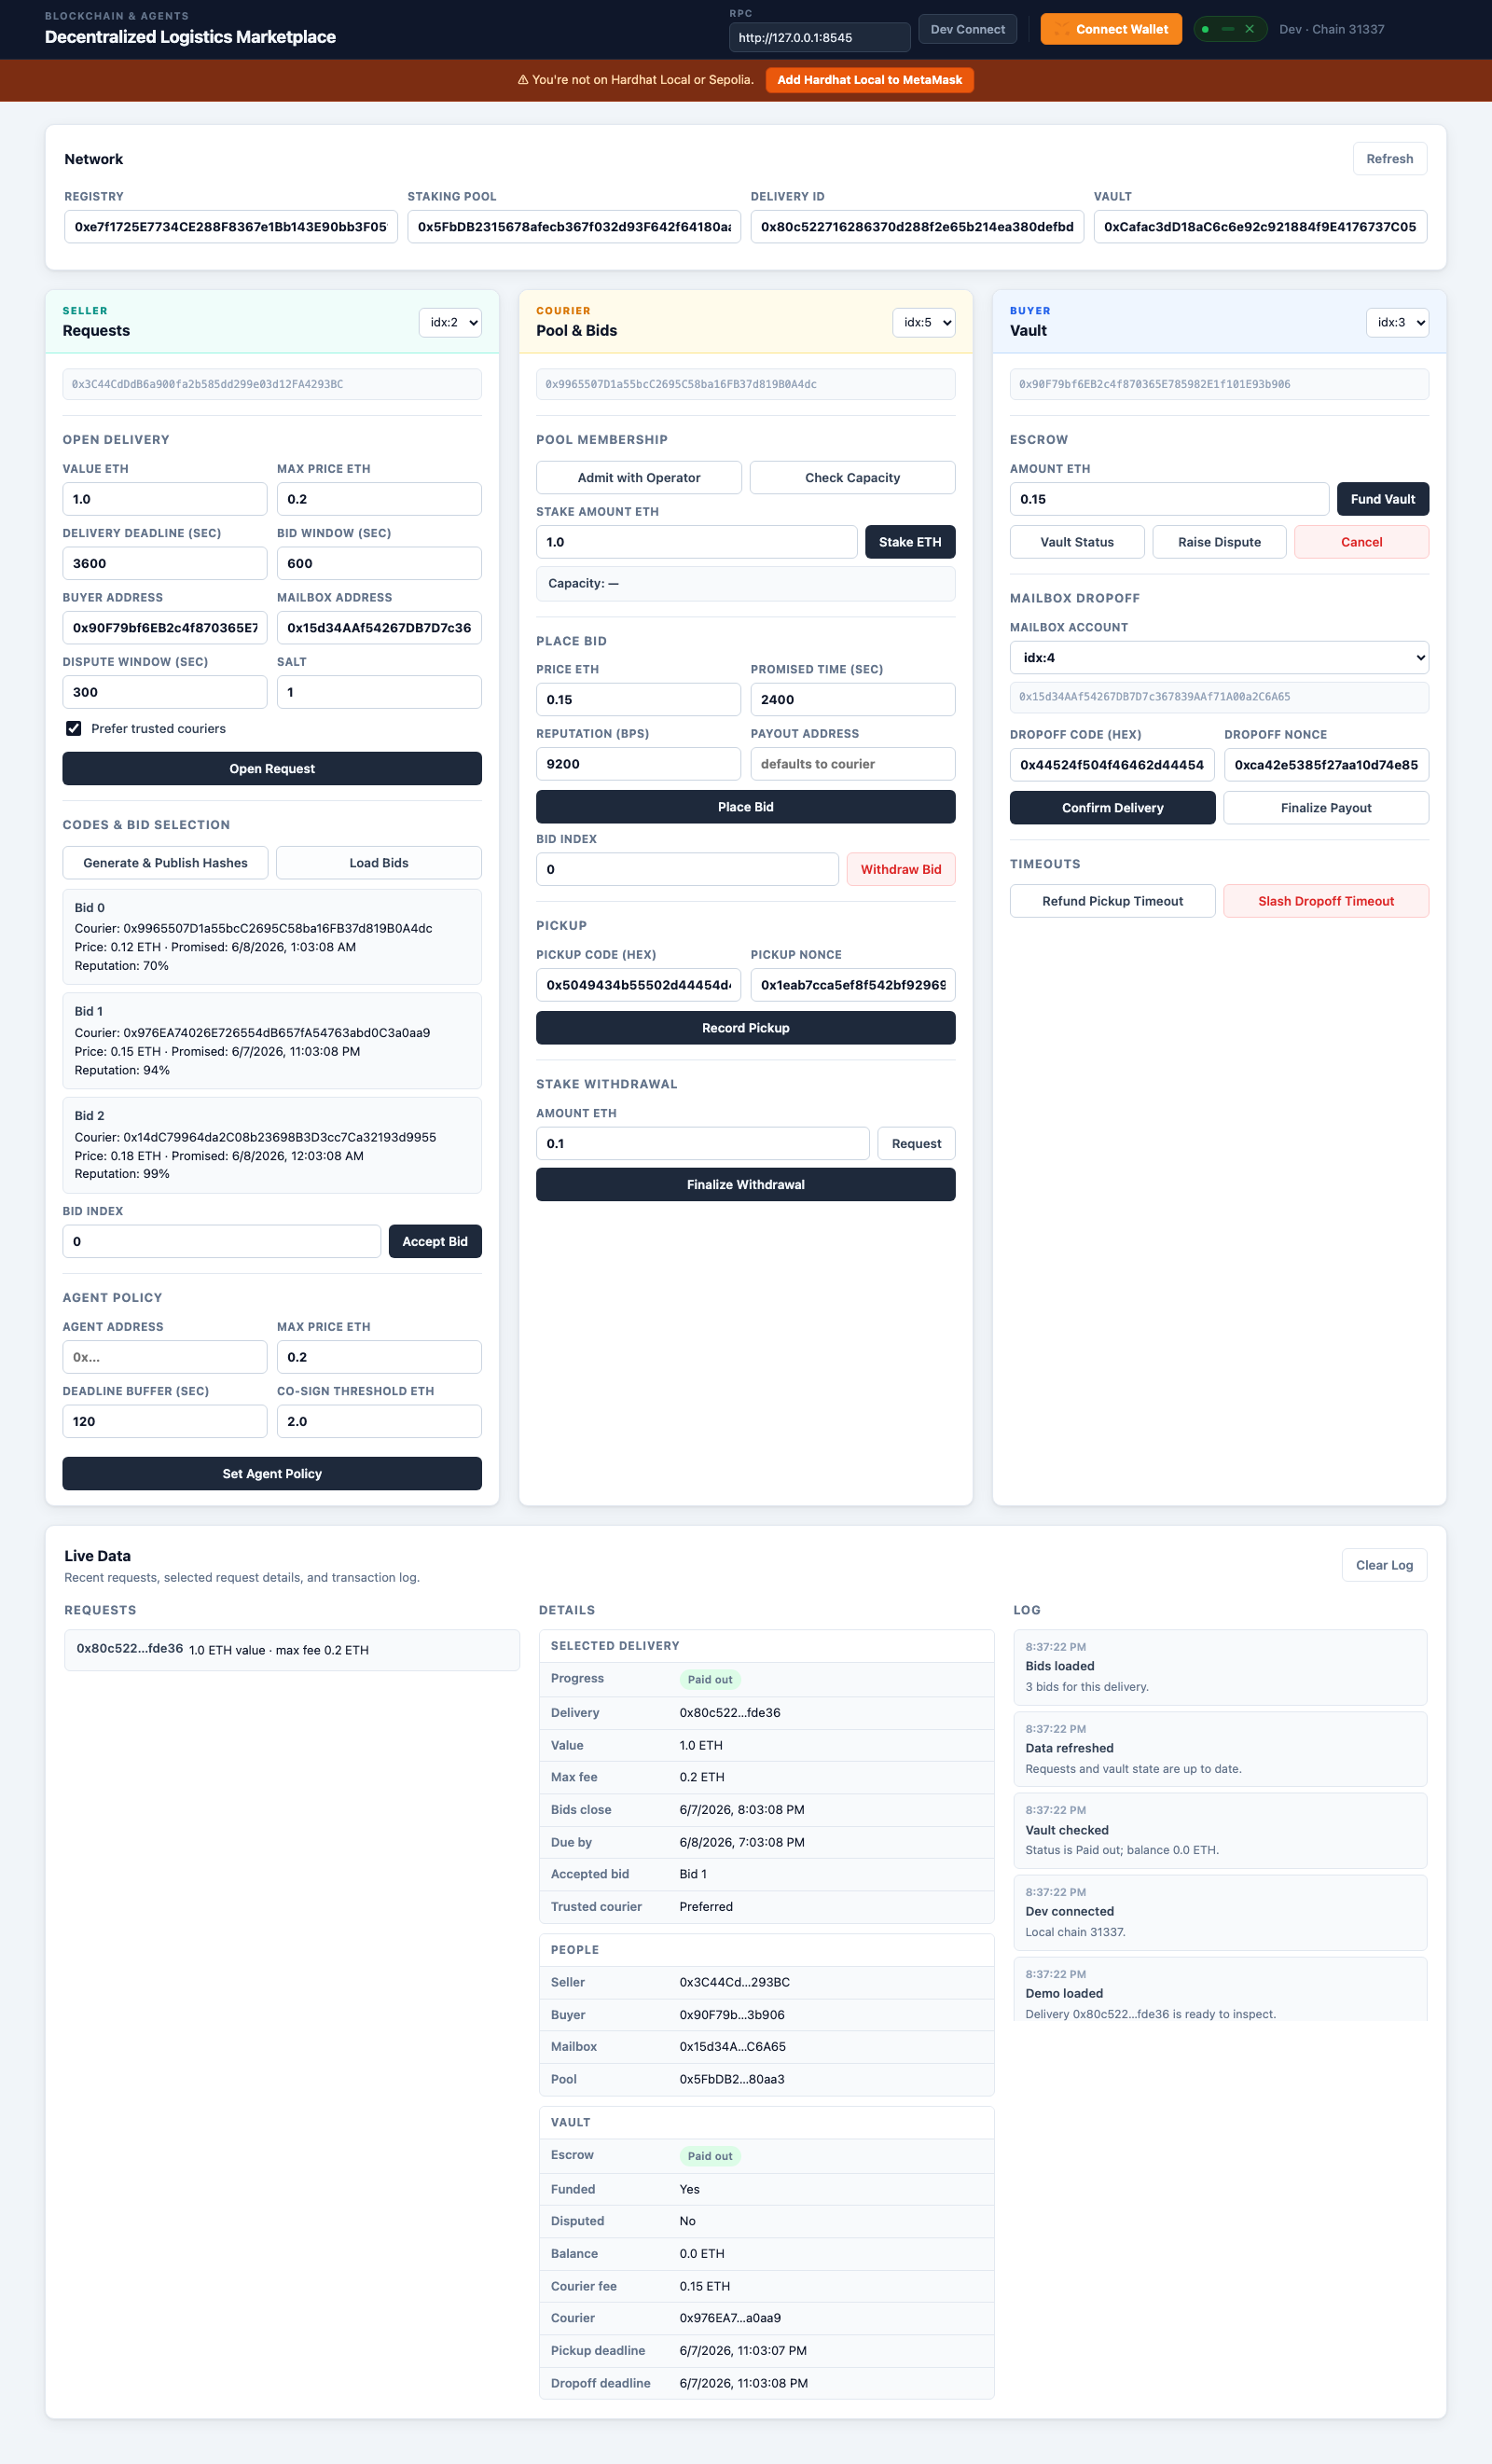
\includegraphics[width=\linewidth]{../test/screenshots/12-full-ui.png}
    \caption{Full DLM Console UI — all three role panels (Seller, Courier, Buyer), Live Data section, and transaction log. Screenshot taken from Playwright test 12.}
    \label{fig:fullui}
\end{figure}

\begin{figure}[H]
    \centering
    \begin{subfigure}[b]{0.48\linewidth}
        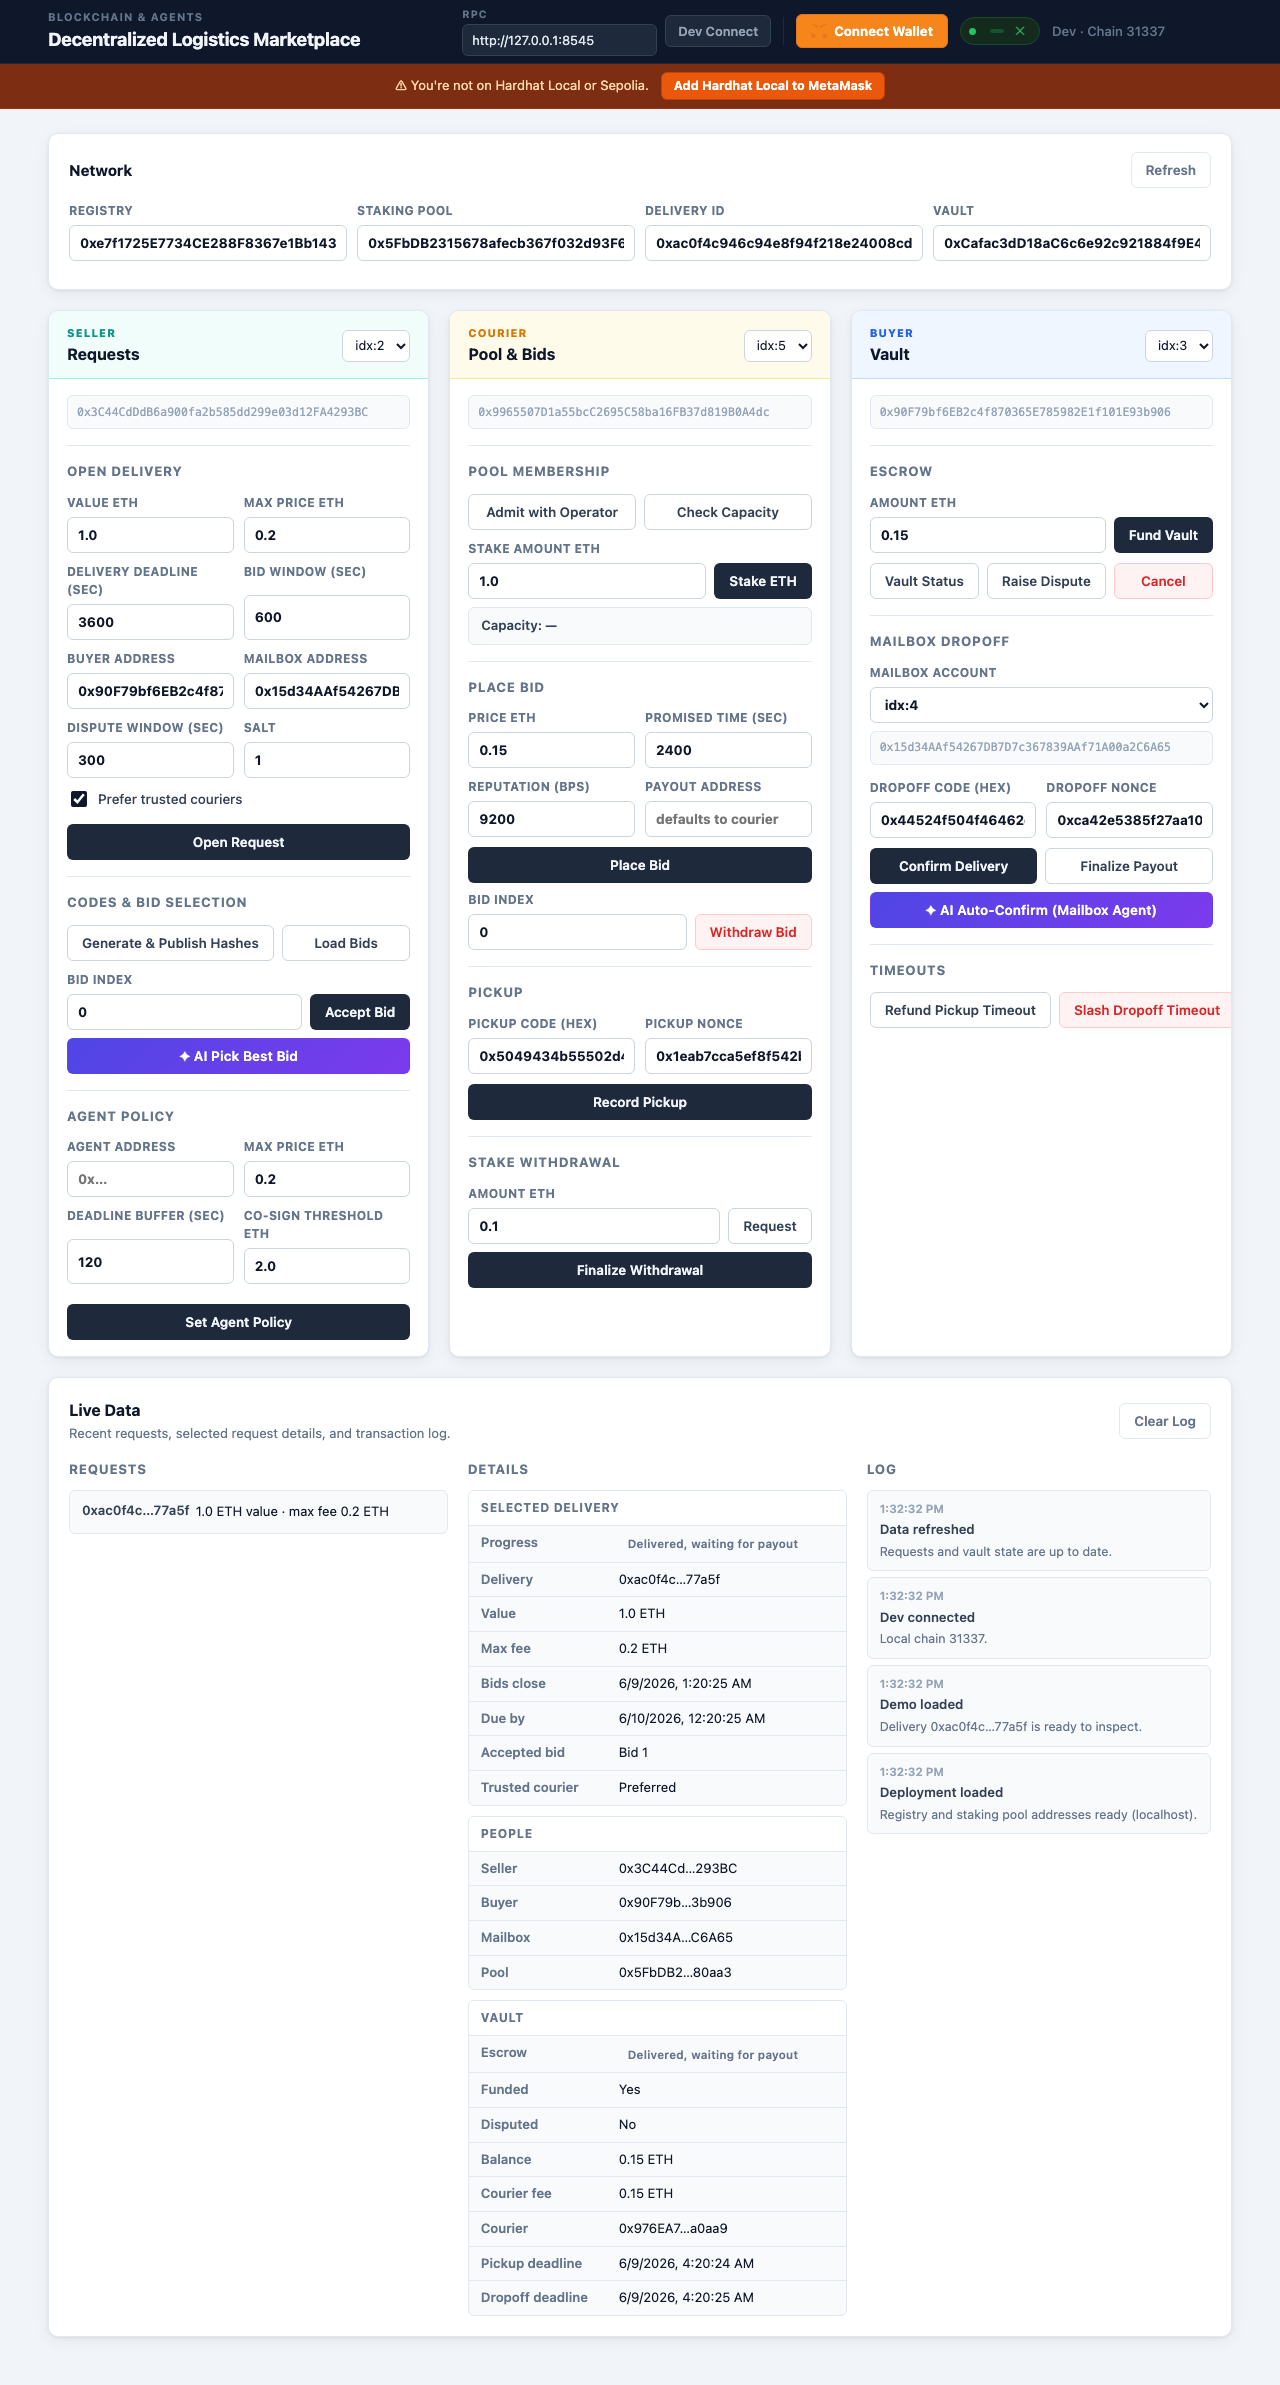
\includegraphics[width=\linewidth]{../test/screenshots/05-requests-list.png}
        \caption{Requests panel showing on-chain delivery requests.}
    \end{subfigure}
    \hfill
    \begin{subfigure}[b]{0.48\linewidth}
        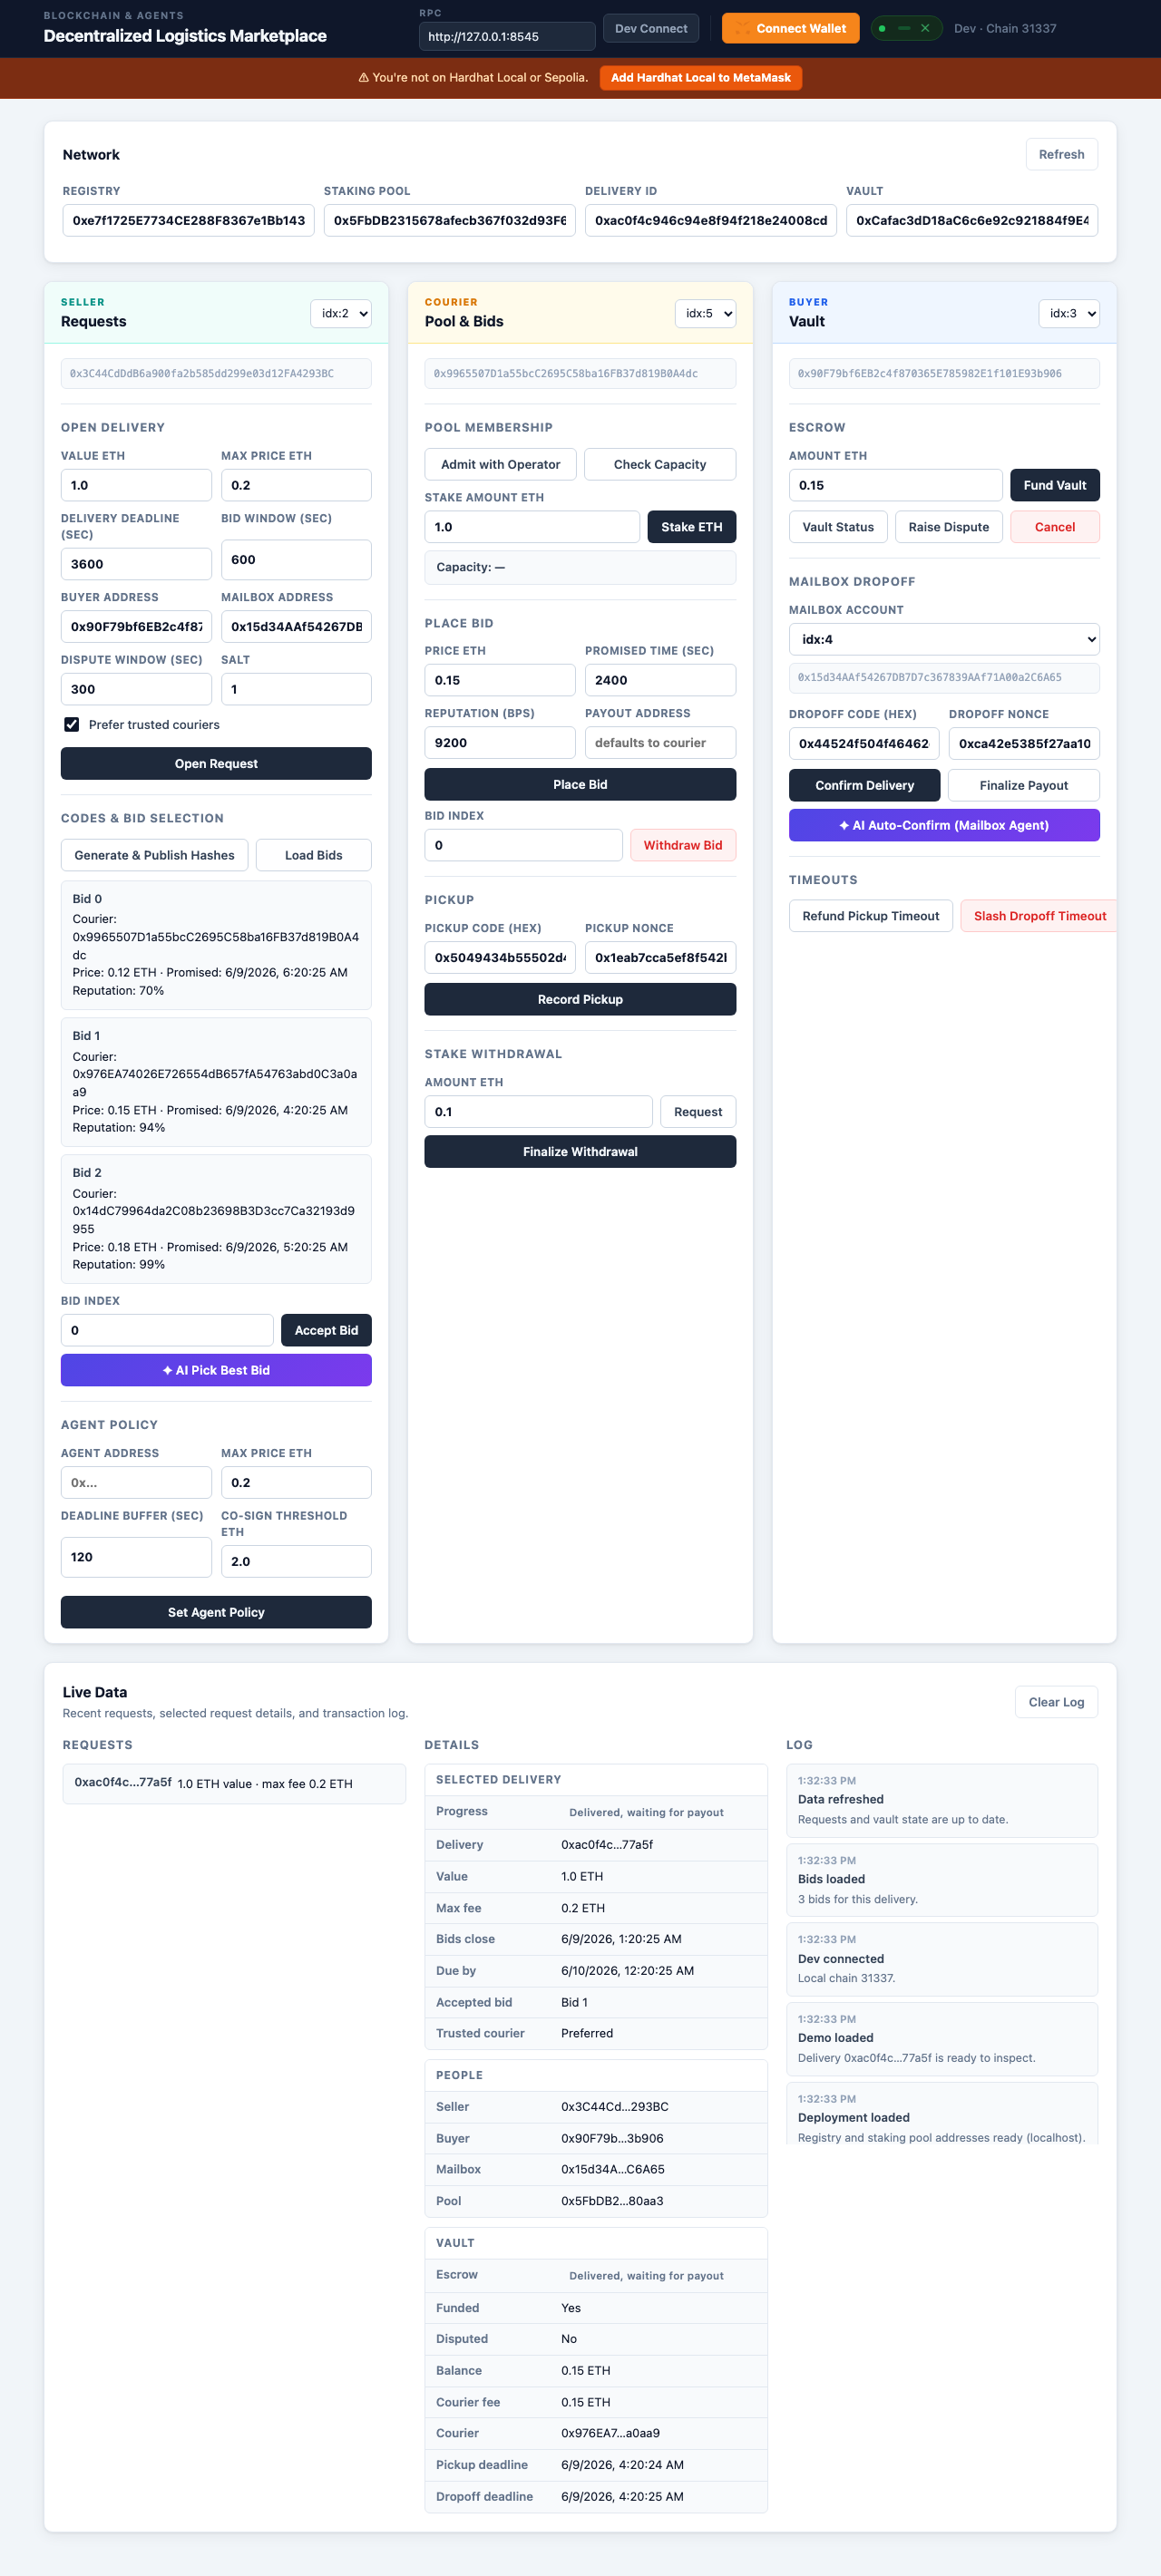
\includegraphics[width=\linewidth]{../test/screenshots/08-bids-loaded.png}
        \caption{Bids panel after loading courier bids for the demo delivery.}
    \end{subfigure}
    \caption{Live data panels populated from on-chain state.}
    \label{fig:panels}
\end{figure}

\begin{figure}[H]
    \centering
    \begin{subfigure}[b]{0.48\linewidth}
        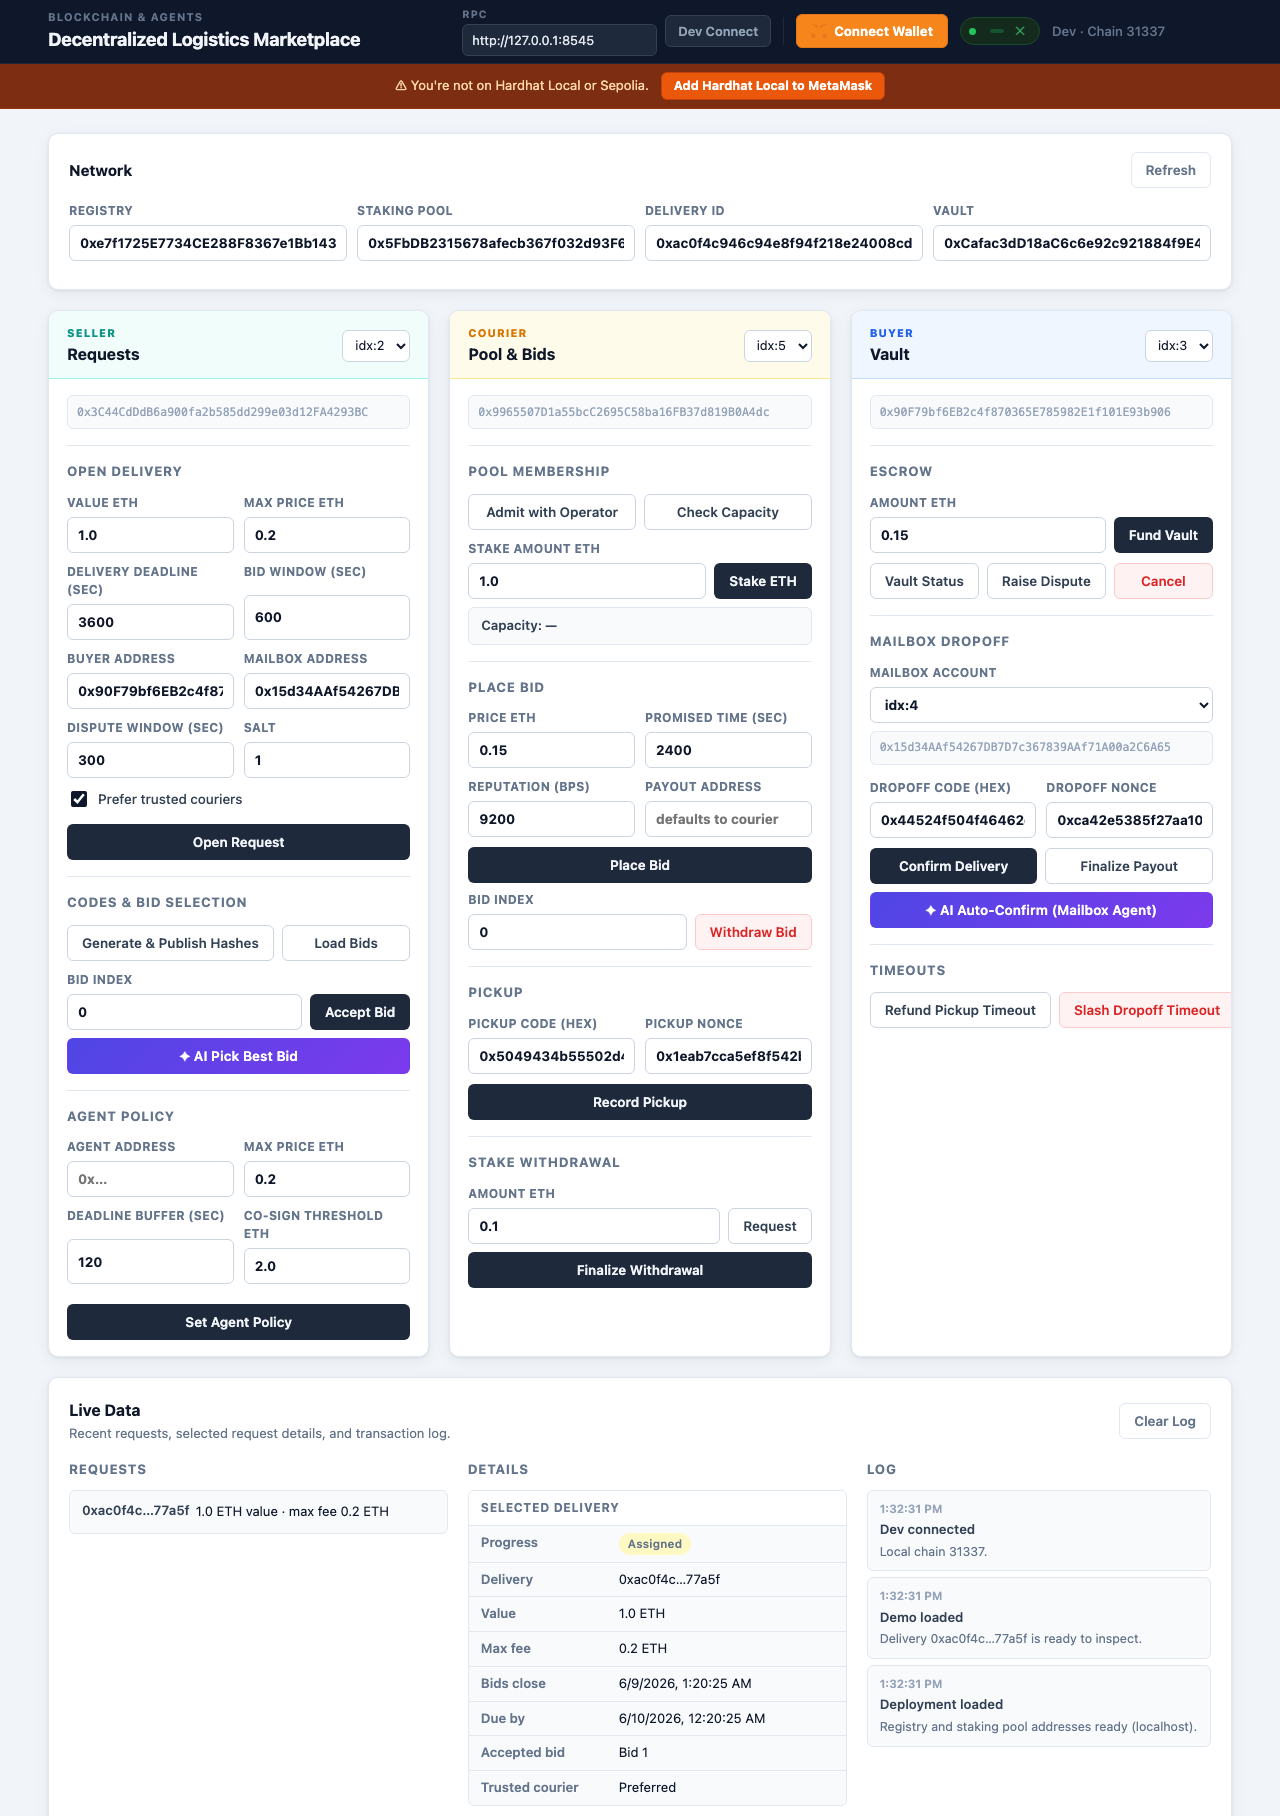
\includegraphics[width=\linewidth]{../test/screenshots/02-connected.png}
        \caption{Connected to Hardhat Local (chain 31337).}
    \end{subfigure}
    \hfill
    \begin{subfigure}[b]{0.48\linewidth}
        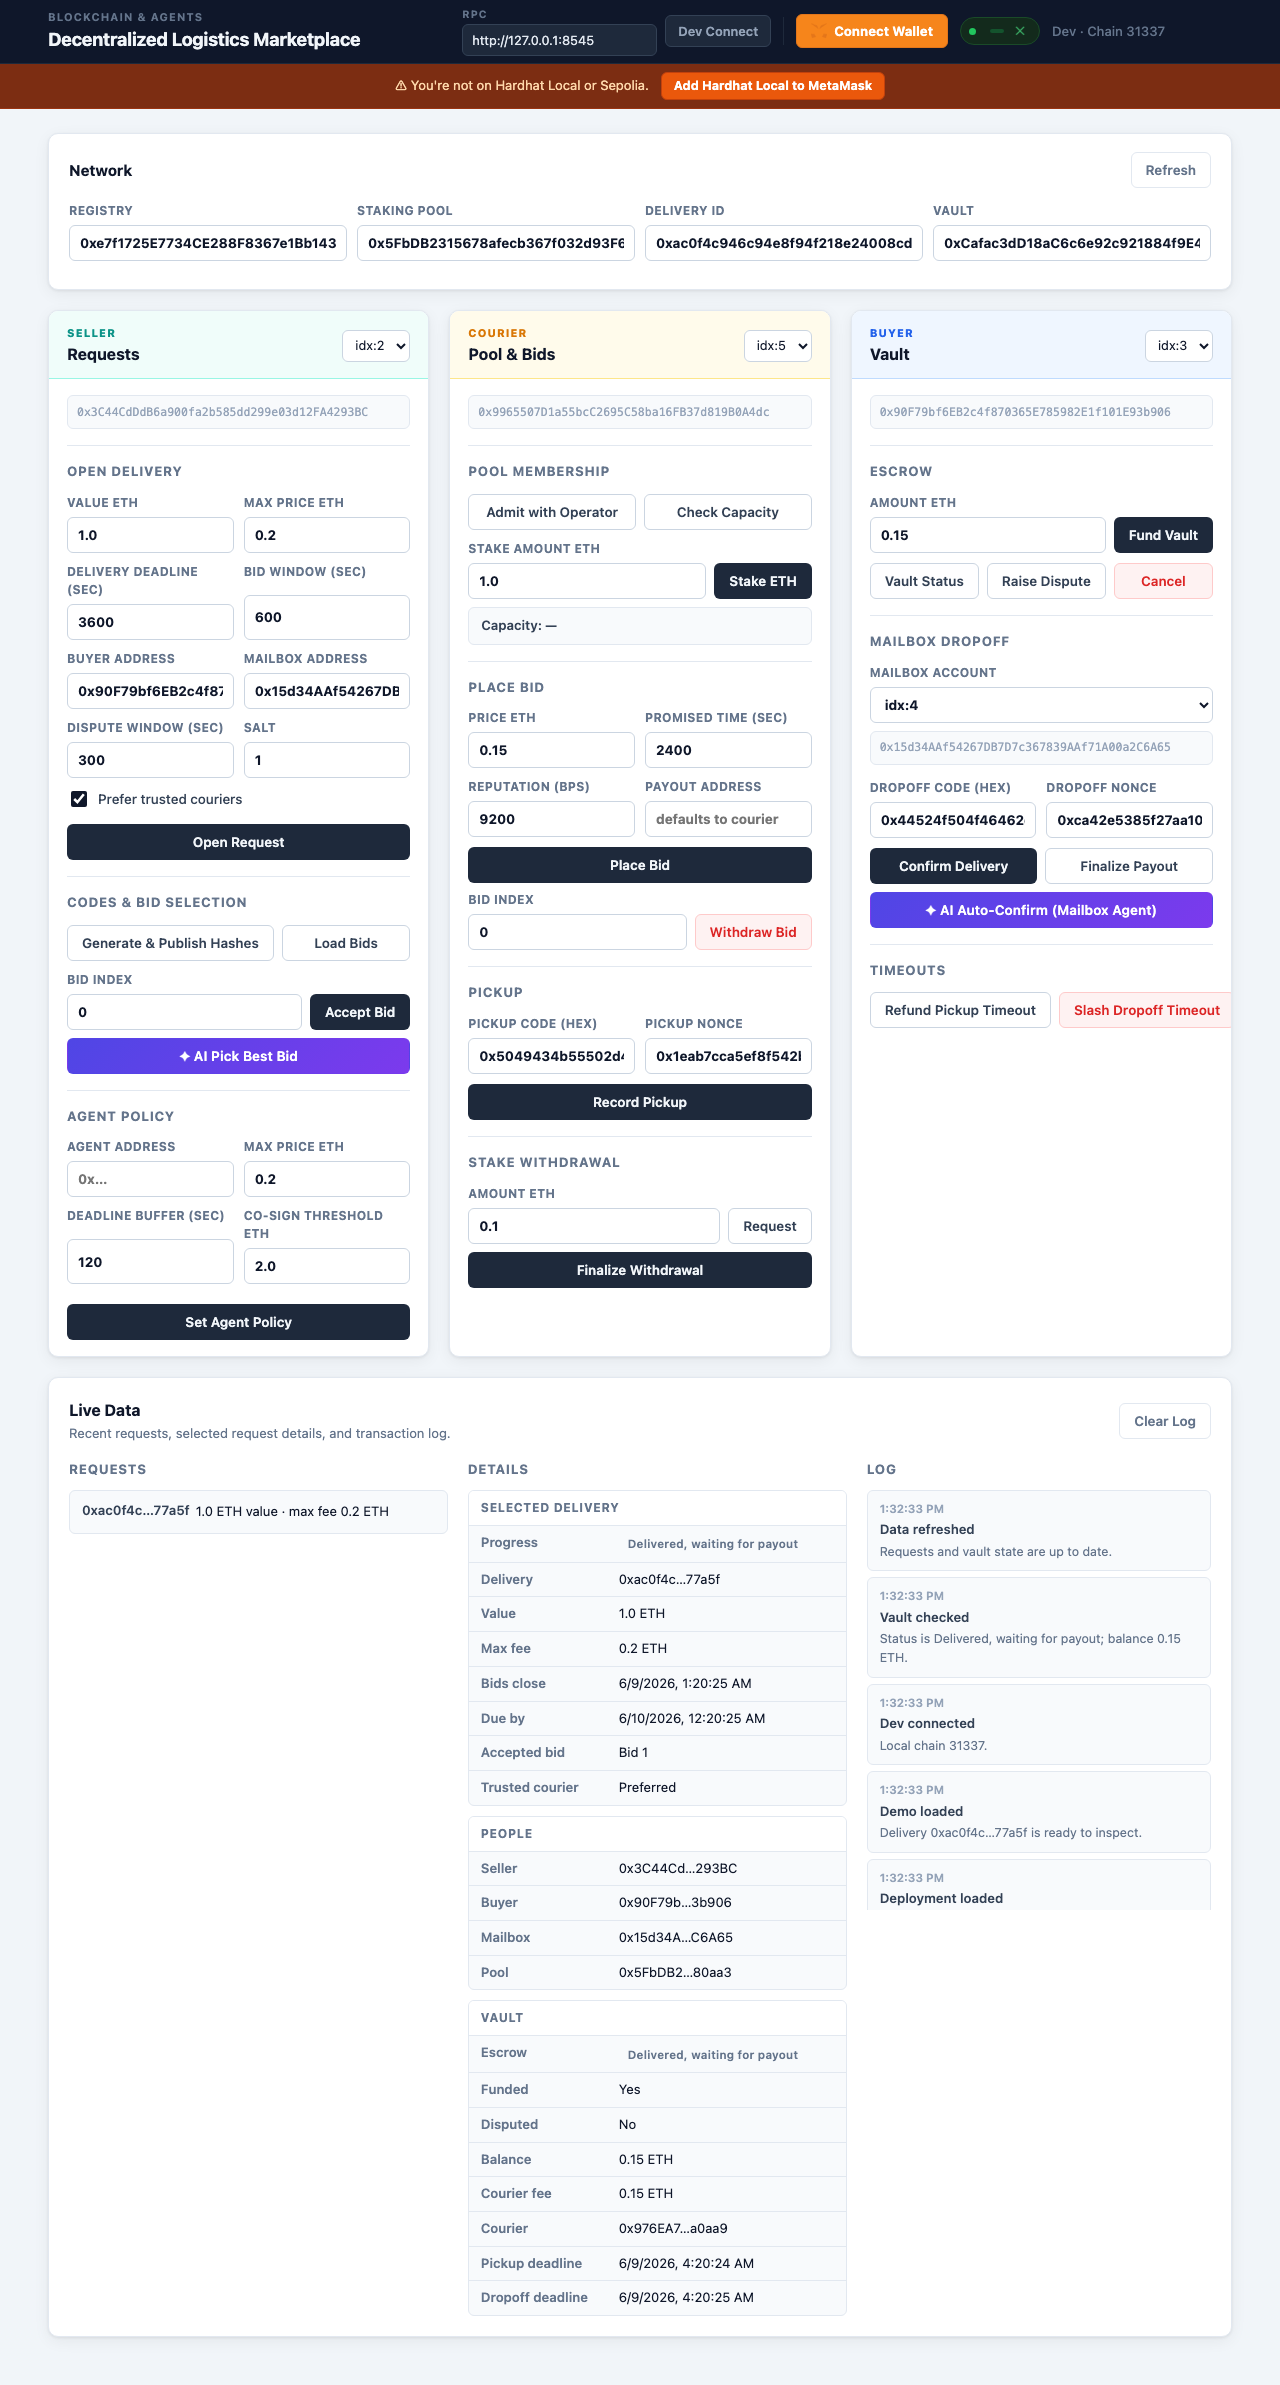
\includegraphics[width=\linewidth]{../test/screenshots/07-vault-status.png}
        \caption{Vault status check showing Delivered, waiting for payout state.}
    \end{subfigure}
    \caption{Connection and vault status screens.}
    \label{fig:connection}
\end{figure}

\subsection{AI Agent Buttons}

The frontend exposes two AI-assisted actions that call the server-side agent API, both powered by the OpenAI GPT-4o-mini model.

\subsubsection{AI Pick Best Bid}

Calls \texttt{POST /api/agent/rank} with the loaded bids. The server runs the deterministic \texttt{SellerAgent.rank()} formula, then sends the bids and winner to GPT-4o-mini for a plain-English explanation. The bid index auto-fills and the explanation appears in a purple card below the bids list.

\begin{figure}[H]
    \centering
    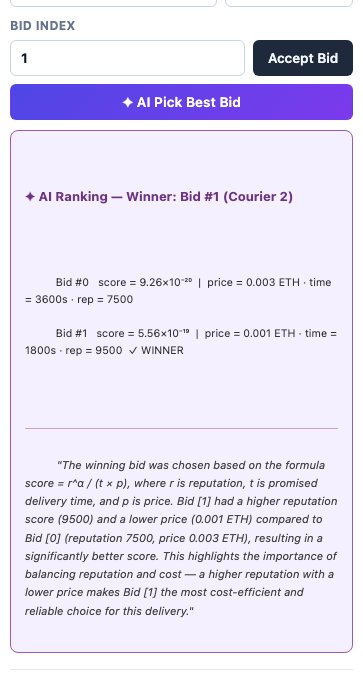
\includegraphics[width=0.55\linewidth]{screenshots/ai-pick-bid-ui.png}
    \caption{\textbf{✦ AI Pick Best Bid} button (purple) in the Seller panel. After clicking, GPT-4o-mini explains the winning bid selection.}
    \label{fig:aipick}
\end{figure}

\textbf{Sample GPT-4o-mini response} (two courier bids: Courier~1 at 0.003~ETH / 3600~s / rep~7500, Courier~2 at 0.001~ETH / 1800~s / rep~9500):

\begin{mdframed}[backgroundcolor=blue!4, linecolor=blue!30]
\small\itshape
``The winning bid was chosen based on the formula score = $r^\alpha$ / ($t \times p$), where $r$ represents the reputation score, $t$ is the promised time, and $p$ is the price. Bid~[1] had a higher reputation score (9500) and a lower price (0.001~ETH) compared to Bid~[0] (reputation 7500 and price 0.003~ETH), which resulted in a more favourable score when applying the formula, despite both bids having similar promised times. This highlights the importance of balancing reputation and cost; a higher reputation can sometimes offset the differences in promised time, making it a more appealing choice overall for the logistics marketplace. Therefore, Bid~[1] was chosen as the winning bid due to its better overall score calculation.''
\end{mdframed}

\subsubsection{AI Auto-Confirm (Mailbox Agent)}

Calls \texttt{POST /api/agent/mailbox-confirm}. The server reads simulated sensor data (package weight, lid state), passes it to GPT-4o-mini for a delivery decision, and — if the AI confirms — submits \texttt{confirmDelivery(code, nonce)} on-chain using the dedicated \texttt{MAILBOX\_KEY}. The AI reasoning and sensor readings appear in the transaction log.

\begin{figure}[H]
    \centering
    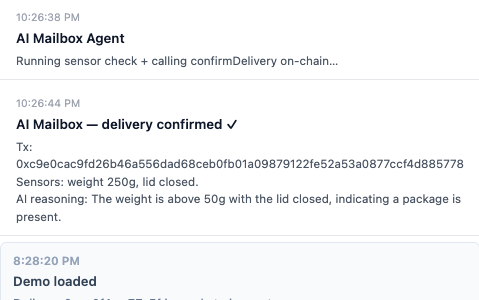
\includegraphics[width=0.55\linewidth]{screenshots/ai-mailbox-ui.png}
    \caption{Transaction log output from the \textbf{✦ AI Auto-Confirm (Mailbox Agent)} after a successful confirmation. GPT-4o-mini sensor reasoning, the on-chain tx hash, and sensor readings are all visible.}
    \label{fig:aimailbox}
\end{figure}

\textbf{Sample GPT-4o-mini response} (sensor reading: weight = 250~g, lid = closed):

\begin{mdframed}[backgroundcolor=blue!4, linecolor=blue!30]
\small\itshape
``The weight is above 50g with the lid closed, indicating a package is present.''
\end{mdframed}

The full log entry produced by the frontend after a successful mailbox confirmation:

\begin{lstlisting}[language=bash, numbers=none, caption=Mailbox Agent log output]
AI Mailbox -- delivery confirmed
Tx: 0xc9e0cac9fd26b46a556dad68ceb0fb01a098791...
Sensors: weight 250g, lid closed.
AI reasoning: The weight is above 50g with the lid closed,
indicating a package is present.
\end{lstlisting}

% =============================================================================
\section{Testnet Deployment}
% =============================================================================

Both contracts are deployed and verified on the Ethereum Sepolia testnet.

\begin{center}
\begin{tabular}{ll}
\toprule
Contract & Sepolia Address \\
\midrule
\texttt{StakingPool} & \texttt{0xD3a16FA31Df5054fA62212FCae16f81AF945bEA2} \\
\texttt{MarketplaceRegistry} & \texttt{0x526B503aaF9dFc75c612FD383A6AAA4C85578237} \\
\bottomrule
\end{tabular}
\end{center}

Contracts can be inspected on \href{https://sepolia.etherscan.io/address/0xD3a16FA31Df5054fA62212FCae16f81AF945bEA2}{Sepolia Etherscan}. \texttt{DeliveryVault} instances are deployed on-demand by the registry when a bid is accepted; each has its own address.

\begin{figure}[H]
    \centering
    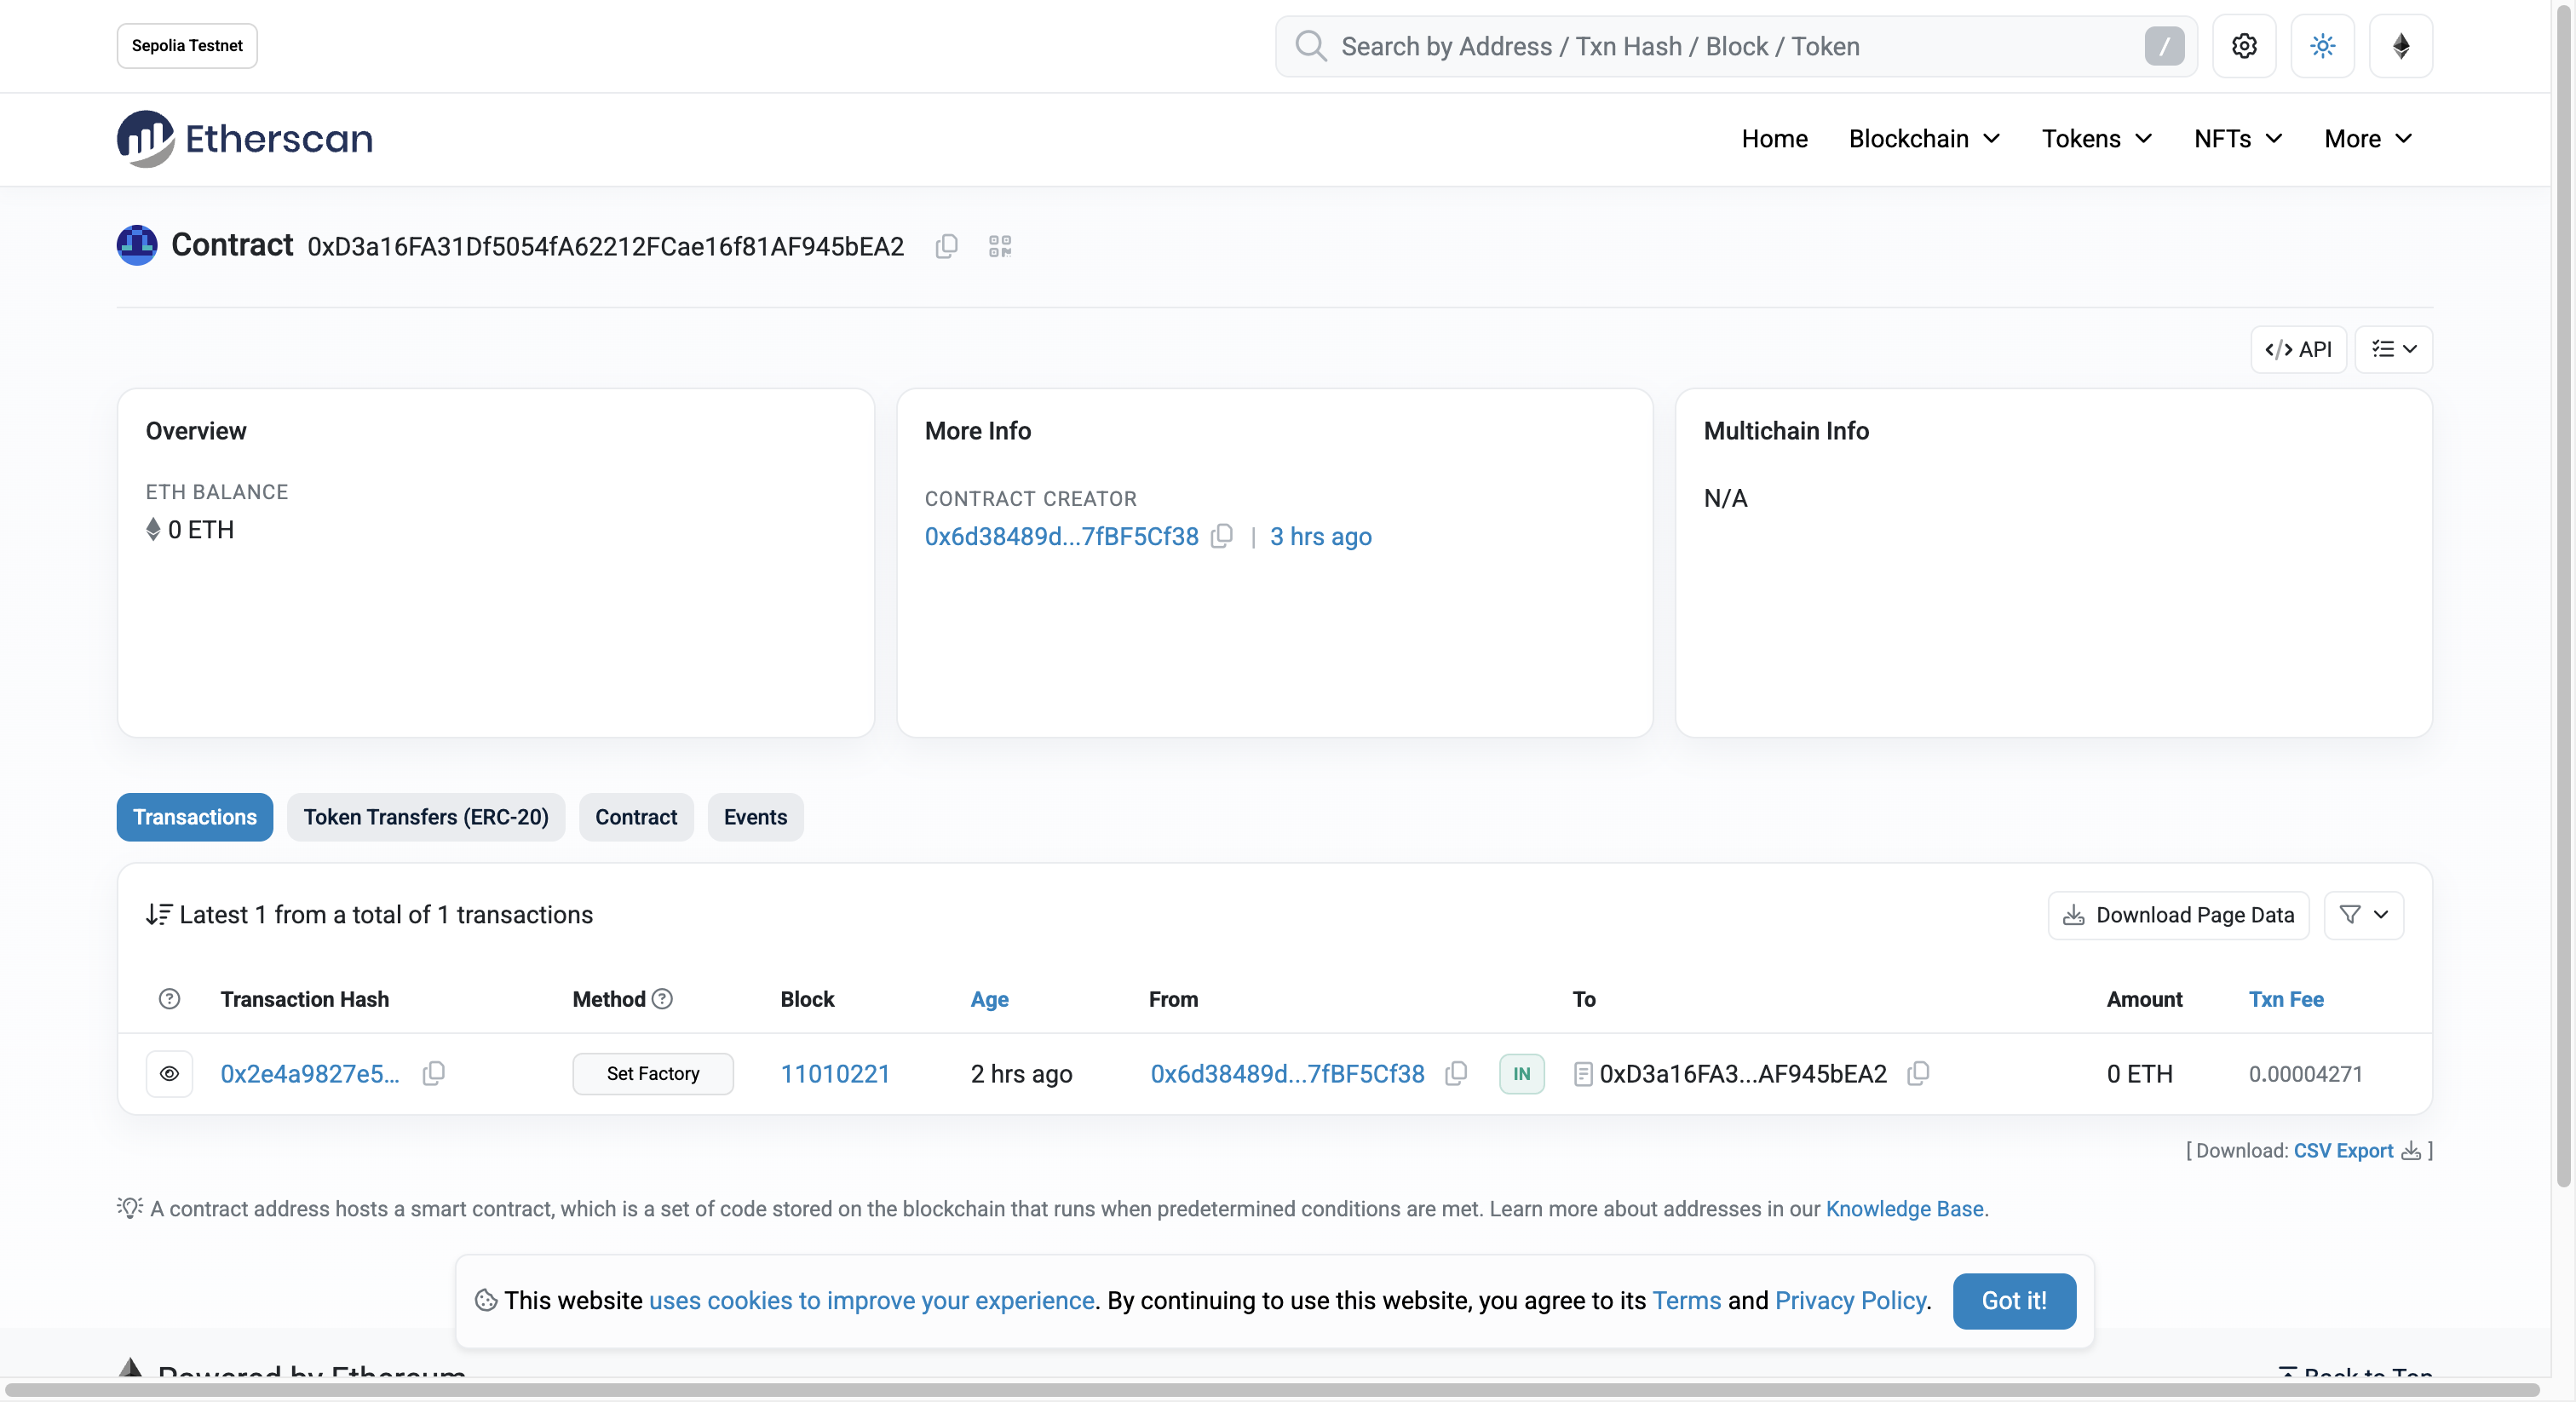
\includegraphics[width=\linewidth]{screenshots/etherscan-sepolia.png}
    \caption{Sepolia Etherscan showing verified on-chain transactions for the \texttt{MarketplaceRegistry} contract, including open request, publish hashes, accept bid, and finalize events from live demo runs.}
    \label{fig:etherscan}
\end{figure}

The frontend automatically loads the correct deployment file based on the connected chain ID: \texttt{deployment.11155111.json} for Sepolia, \texttt{deployment.json} for local Hardhat.

% =============================================================================
\section{How to Run}
% =============================================================================

\subsection{Prerequisites}

Node.js 18+, npm.

\begin{lstlisting}[language=bash, numbers=none]
git clone <repo-url>
cd 438proje
npm install
\end{lstlisting}

\subsection{Compile and Test}

\begin{lstlisting}[language=bash, numbers=none]
npx hardhat compile       # compiles all 3 contracts
npx hardhat test test/Marketplace.test.js   # 14 tests
\end{lstlisting}

\subsection{Local End-to-End Demo}

\begin{lstlisting}[language=bash, numbers=none]
# Terminal 1 — start local chain
npm run node

# Terminal 2 — deploy contracts and run full delivery flow
npm run deploy:local
npm run demo
\end{lstlisting}

The demo script runs the complete lifecycle: deploy $\to$ admit couriers $\to$ stake $\to$ open request $\to$ publish hashes $\to$ place bids $\to$ agent ranks and accepts $\to$ buyer funds $\to$ courier picks up $\to$ mailbox confirms $\to$ finalize. Final pool state (totalStake, activeValue) is printed at each step.

\subsection{Frontend GUI}

\begin{lstlisting}[language=bash, numbers=none]
npm run demo:frontend     # seeds a demo delivery into frontend-demo.json
npm run frontend          # serves http://127.0.0.1:5173
\end{lstlisting}

Open \texttt{http://127.0.0.1:5173} in the browser and click \textbf{Dev Connect}.

\subsection{Playwright UI Tests}

\begin{lstlisting}[language=bash, numbers=none]
npx playwright test       # 12 automated end-to-end UI tests
\end{lstlisting}

\subsection{Testnet Deployment}

\begin{lstlisting}[language=bash, numbers=none]
cp .env.example .env      # fill SEPOLIA_RPC_URL and DEPLOYER_KEY
npm run deploy:sepolia    # deploys to Sepolia, writes deployment.11155111.json
\end{lstlisting}

\subsection{Running the Agents}

\begin{lstlisting}[language=bash, numbers=none]
# Seller agent watches a delivery until bid deadline, then auto-accepts
RPC_URL=http://127.0.0.1:8545 AGENT_KEY=idx:6 \
  node agents/seller_agent.js watch <deliveryId> 0.2 false

# Mailbox agent confirms a delivered vault
RPC_URL=http://127.0.0.1:8545 MAILBOX_KEY=idx:4 \
  node agents/mailbox_agent.js confirm <vaultAddr> <code> <nonce>

# A2A listener mode
node agents/seller_agent.js a2a-listen
\end{lstlisting}

% =============================================================================
\section{Project File Structure}
% =============================================================================

\begin{lstlisting}[numbers=none]
438proje/
  contracts/
    MarketplaceRegistry.sol   open requests, bids, agent policy, vault factory
    DeliveryVault.sol         per-delivery escrow, preimage binding, dispute window
    StakingPool.sol           shared collateral, capacity invariant, slashing
  test/
    Marketplace.test.js       14 Hardhat tests (full lifecycle + all attacks)
    ui-demo.spec.js           12 Playwright UI tests
  scripts/
    deploy.js                 deploys pool + registry; writes deployment.json
    demo-end-to-end.js        runs complete lifecycle against a fresh chain
    frontend-demo.js          seeds frontend-demo.json for the GUI demo
  agents/
    seller_agent_core.js      deterministic r/(t*p) bid ranker (no LLM)
    seller_agent.js           watcher + A2A protocol + optional Claude commentary
    mailbox_agent.js          sensor simulator, rate-limit, confirmDelivery
  clients/
    seller/seller_cli.js      seller command-line interface
    courier/courier_cli.js    courier command-line interface
    buyer/buyer_cli.js        buyer command-line interface
  frontend/
    index.html                main UI (MetaMask + dev mode)
    app.js                    ethers.js v6 frontend logic
    styles.css                professional dark-topbar UI
    server.js                 Node.js HTTP server + /api/agent/* endpoints
  docs/
    A2A.md                    Agent-to-Agent wire protocol schema
    SECURITY.md               attack-by-attack code line references
    REPORT.md                 this report (markdown version)
    report.tex                this report (LaTeX source)
\end{lstlisting}

% =============================================================================
\section{Conclusion}
% =============================================================================

We have built a complete, working decentralized logistics marketplace that enforces all critical payment guarantees in Solidity, on an EVM-compatible chain. The key contributions are:

\begin{enumerate}
    \item A three-contract architecture where \emph{no central party} can alter payment flows after a bid is accepted.
    \item On-chain agent policy enforcement: the seller pre-registers constraints that revert any agent transaction violating them, making LLM hallucination economically inert.
    \item A staking pool that maintains $\texttt{activeValue} \leq \texttt{totalStake}$ as a hard invariant on every state transition.
    \item Preimage-bound pickup/dropoff codes that prevent code replay across deliveries.
    \item A sensor-gated, rate-limited mailbox agent that bridges the physical-world delivery to on-chain payment release.
    \item 14 Hardhat tests covering the full happy path and every documented attack, plus 12 Playwright UI tests providing automated end-to-end demo coverage.
    \item Live testnet deployment on Ethereum Sepolia.
\end{enumerate}

The system is reproducible: a fresh machine can run \texttt{npm install \&\& npx hardhat test} and see all 14 tests pass in under 30 seconds.

\end{document}
